\documentclass[10pt]{report}
\usepackage{graphicx}
%\usepackage[ruled,vlined]{algorithm2e}
\usepackage[]{algorithm2e}
\usepackage{subcaption}
%\usepackage{subfig}


\graphicspath{{../Figures/}}		% path to graphic files
\usepackage{fullpage}
%\usepackage{fancyhdr}
%\rhead{
%\includegraphics[width=\textwidth]{header}
%}
%\lhead{
%\includegraphics[width=\textwidth]{header}
%}
  \usepackage[dvipsnames]{xcolor}
  \usepackage{tikz}
\usepackage{verbatim}

\usepackage{bbding} 

\usepackage[most]{tcolorbox}
\newtcblisting{commandshell}{colback=black,colupper=white,
listing only,listing options={style=tcblatex,language=sh},
every listing line={\textcolor{green}{\small\ttfamily\bfseries  \$ }}}


\usepackage{bm}
\usepackage{amsmath}
\usepackage{amssymb}
\usepackage{amsthm} 
%\usepackage{wrapfig} 
%\usepackage[percent]{overpic}

\usepackage{natbib} 
\usepackage{lipsum}


\usepackage[pagebackref]{hyperref}
\hypersetup{
   % pagebackref =true,
    colorlinks,%
    citecolor=blue,% 
    filecolor=black,%
    linkcolor=magenta,% 
    urlcolor=black
}

  
%\author{Giacomo Po}
%\title{Field Equations of Discrete Dislocations}


\newcommand{\dL}[0]{\, \text{d}L}
\newcommand{\dA}[0]{\, \text{d}A}
\newcommand{\dV}[0]{\, \text{d}V}

\newcommand{\GP}[0]{G^\Delta}
\newcommand{\hGP}[0]{\hat{G}^\Delta}

\newcommand{\GH}[0]{G^L}
\newcommand{\hGH}[0]{\hat{G}^L}

\newcommand{\bPc}[0]{\beta^{P}}
%\newcommand{\bPg}[0]{\beta^{P}}

%\newcommand{\bEg}[0]{\beta}
\newcommand{\bEc}[0]{\beta}

\newcommand{\eEc}[0]{\varepsilon}
\newtheorem{mytheorem}{Theorem}
\newtheorem{mydefinition}{Definition}



%%%%%%%%%%%%%%%%%%%%%%%%%%%%%%%%%%%%%%%%%%%%
%%%%%%%%%%%%%%%%%%%%%%%%%%%%%%%%%%%%%%%%%%%%
\begin{document}


\thispagestyle{empty}
\begin{tikzpicture}[remember picture,overlay] 
\def \Px{-3.5}
\def \Py{-20}
\def \Lx{1.2*\textwidth}
\def \Ly{10}
\node[opacity=1,inner sep=0pt] at (current page.center){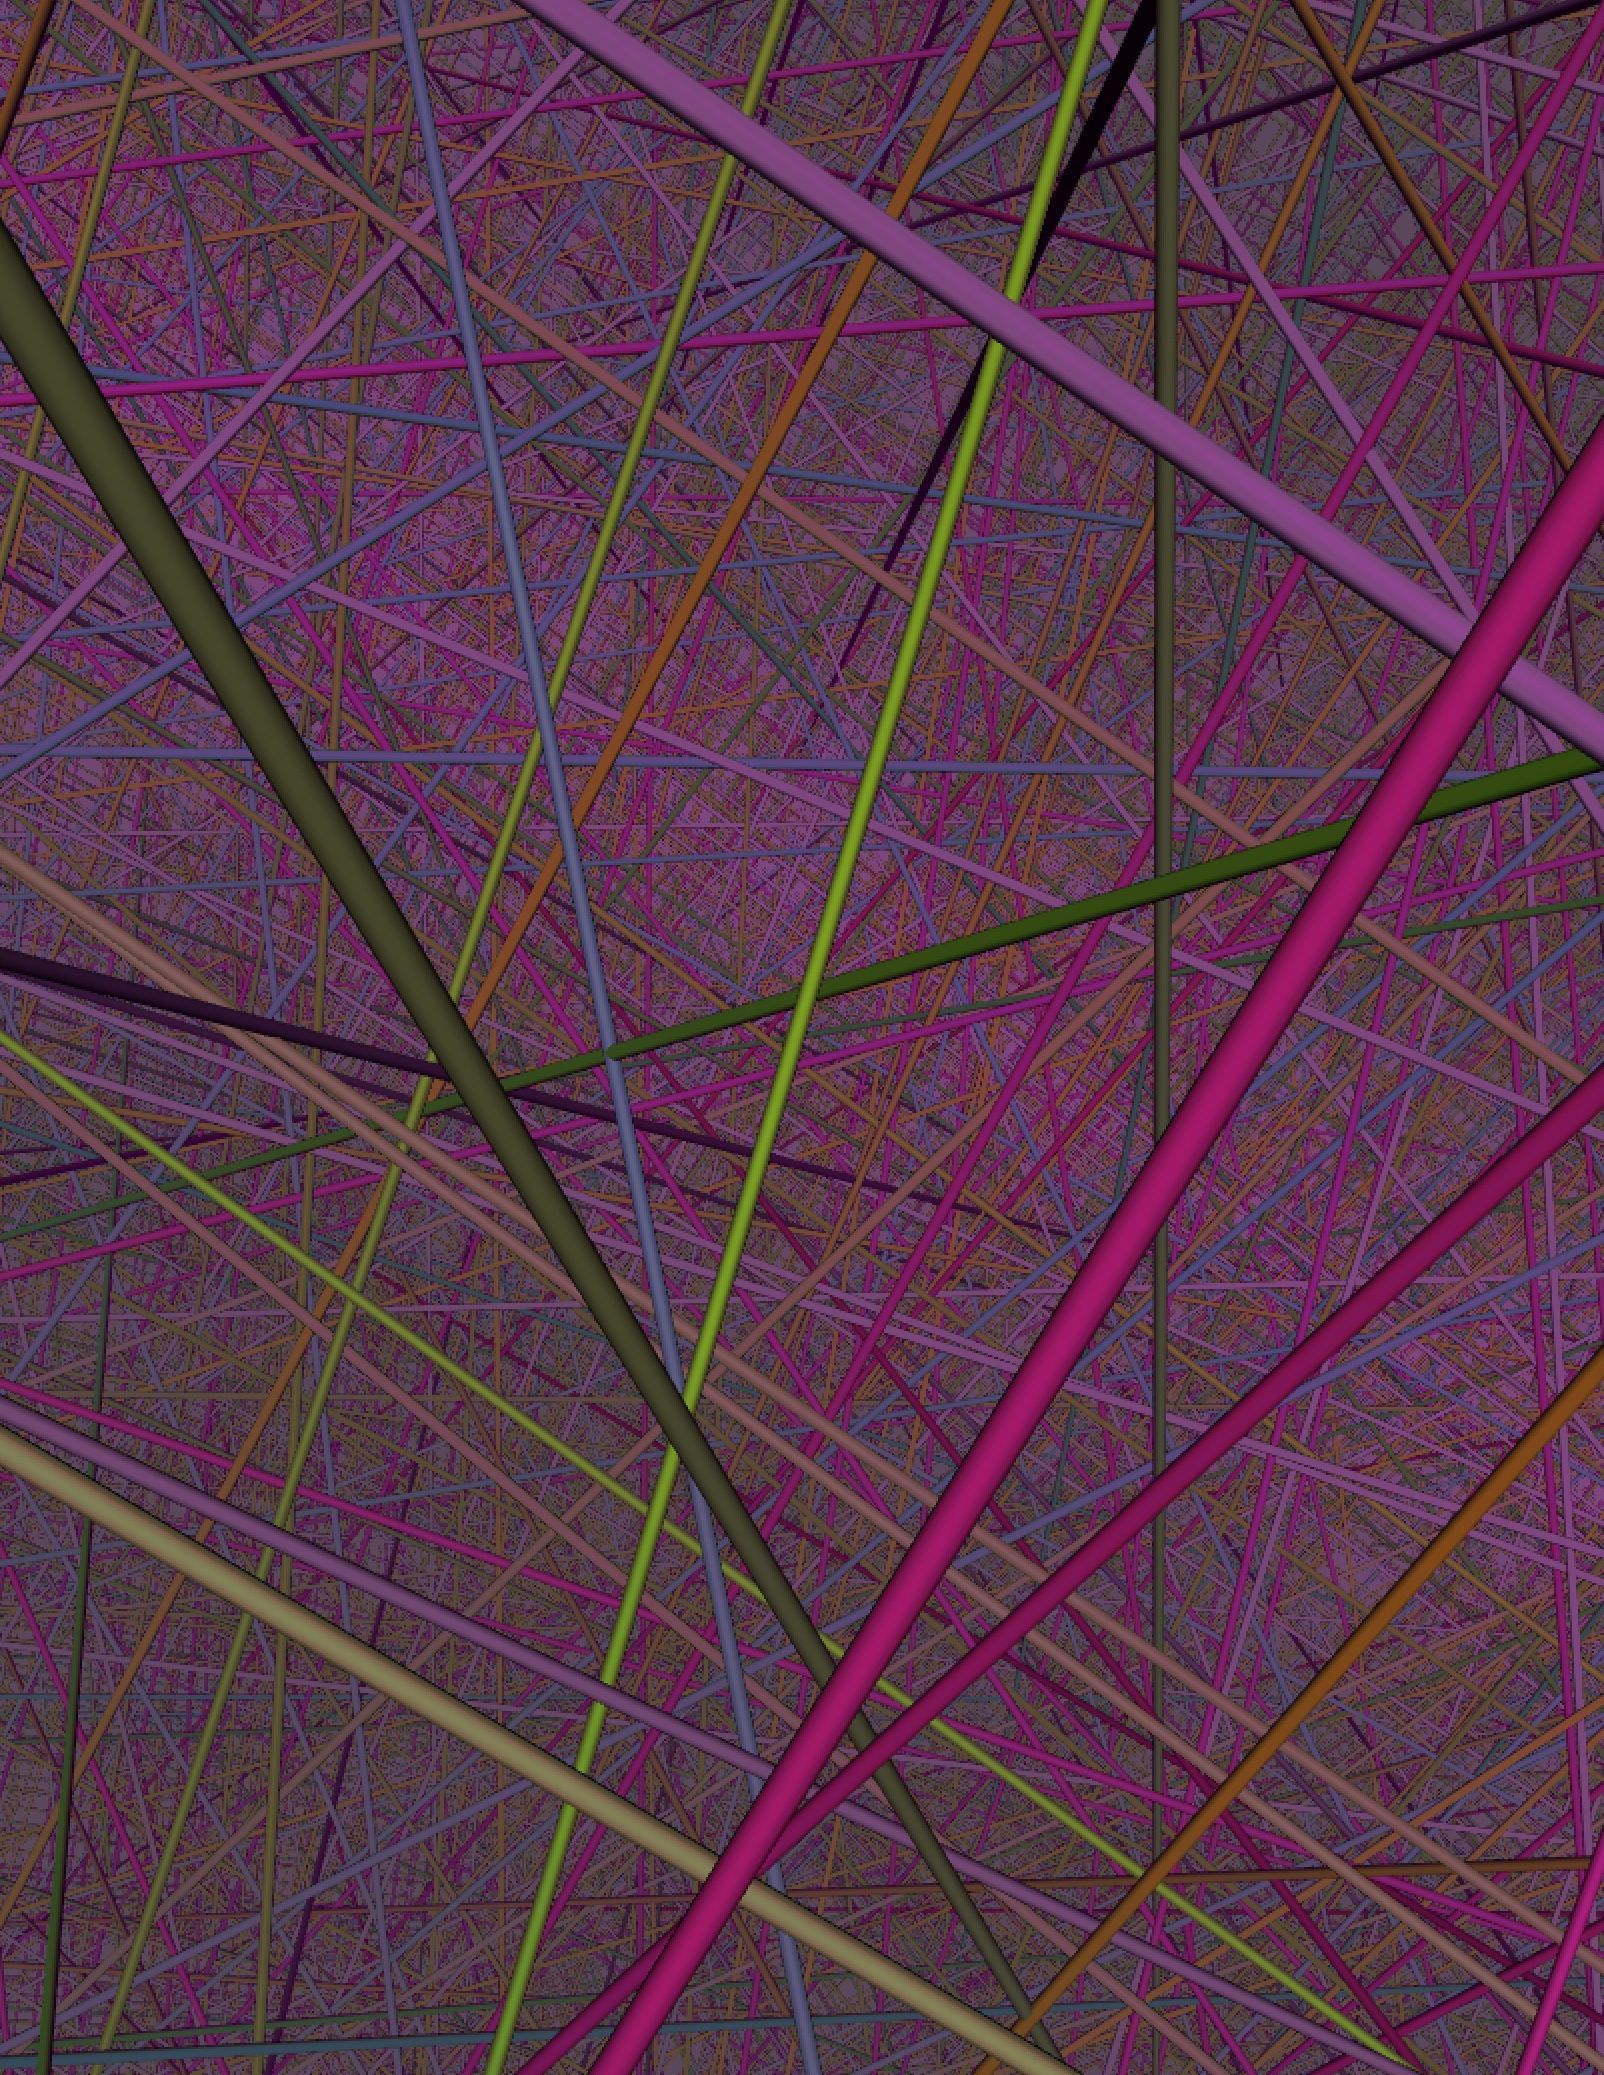
\includegraphics[width=\paperwidth,height=\paperheight]{straight_lines}};
 \fill [black, opacity=0.7]
       (\Px,\Py) -- (\Px,\Py+\Ly) -- (\Px+\Lx,\Py+\Ly)-- (\Px+\Lx,\Py) -- cycle;
\node[anchor=north west] at (\Px+3.0,\Py+\Ly-1) {\Huge{\textcolor{white}{
\textbf{MoDELib manual}}}};
\node[anchor=north west] at (\Px+3.0,\Py+\Ly-2) {\Large{\textcolor{white}{
???}}};
%\node[anchor=north west] at (\Px+3.0,\Py+\Ly-2.8) {\Large{\textcolor{white}{
%}}};

\draw[very thick,orange]  (\Px,\Py+0.4*\Ly) --  (\Px+\Lx,\Py+0.4*\Ly);

\node[anchor=north west] at (\Px+3.0,\Py+\Ly-4) {\Huge{\textcolor{white}{
 ???}}};
\draw[very thick,orange]  (\Px,\Py+0.4*\Ly) --  (\Px+\Lx,\Py+0.4*\Ly);


\node[anchor=north west] at (\Px+3.0,\Py+\Ly-7) {\Huge{\textcolor{white}{
Giacomo Po}}};
\node[anchor=north west] at (\Px+3.0,\Py+\Ly-8) {\Large{\textcolor{white}{
\today}}};
%\node[anchor=north west] at (\Px+4.5,\Py+\Ly-7) {\large{\textcolor{white}{
%10755 Massachusetts Ave}}};
%\node[anchor=north west] at (\Px+4.5,\Py+\Ly-8) {\large{\textcolor{white}{
%Los Angeles, CA}}};
 \end{tikzpicture}

%\maketitle

\chapter*{Preface}
\chapter*{Acknowledgements}
\tableofcontents
\newpage
\chapter{The elastic theory of discrete dislocations\label{elasticTheoryDislocations}}


The key aspect of the DDD method is that dislocation interactions are computed without resorting to expensive atomistic calculations. This is made possible by the 
elastic theory of dislocations, which provides semi-analytical expressions of the elastic fields (displacement, stress, strain\ldots) generated by  arbitrary dislocation loops within an infinite elastic medium. We now briefly summarize this theory,  as a special case of Mura's linearized eigendistortion theory \citep{Mura:1987wt}. 

%%%%%%%%%%%%%%%%%%%%%%%%%%%%%%%%%%%%%%%%%%%
\section{The eigendistortion problem in the infinite elastic medium\label{eigendist_classical}}
Let us consider an elastic body occupying the infinite three-dimensional space $\mathbb{R}^3$, and let $\bm u(\bm x)$ be its displacement field. We adopt here the linearized eigen-distortion framework of \cite{Mura:1987wt}, in which the main kinematic assumption  is that the displacement gradient is split additively into an elastic distortion $\bm \beta$, and an inelastic distortion $\bm \beta^\star$:
\begin{align}
u_{i,j}=\beta_{ij}+\beta^\star_{ij}\, .
\label{linear_decomposition}
\end{align}
The elastic distortion describes the local stretching of the atomic bonds and is related to stress via Hookes law ($\sigma_{ij}=\mathbb{C}_{ijkl}\beta_{kl}$). On the other hand, the inelastic distortion is the \textit{eigendistortion} of  the material, and it may contain several (additive) contributions, including plastic deformation, thermal deformation, deformation due to point defects and diffusive species in the lattice, and more. The inelastic distortion is also referred to as an \textit{eigendistortion}, because it is imagined to take place within a fictitious ``intermediate" configuration where the body is allowed to deform with incompatibilities (separations and/or interpenetrations) in order  to remain stress free. It is the subsequent elastic distortion which is responsible to develop the internal stress field necessary to remove the incompatibilities of the intermediate configuration. It will be shown that an eigendistortion field results in a state of self-stress if it is incompatible, that is if its (negative) curl 
\begin{align}
\alpha_{ij}=-\epsilon_{jkm}\beta^\star_{im,k}
\label{alpha}
\end{align}
is non vanishing. If the eigendistortion is due to dislocations, then $\bm \alpha$ can be interpreted as a tensorial density of dislocations, which  is  known as the Kr\"oner-Nye dislocation density tensor.


%In this document, we consider only the plastic contribution of the inelastic eigendistortion, so that 
%\begin{align}
%\bm\beta^\star=\bm\beta^P\, ,
%\end{align}
%where $\bm\beta^P$ is the plastic distortion caused by dislocations.

 


In the presence of a body forces density $\bm b$, 
the  static Lagrangian density of the classical linear elastic medium reads
\begin{align}
\mathcal{L}&=-\mathcal{W}-\mathcal{V}\nonumber=-\frac{1}{2}\mathbb{C}_{ijkl}\beta_{ij}\beta_{kl}+u_if_i\, ,
\end{align}
where 
\begin{align}
\label{V}
\mathcal{V}=-u_i b_i
\end{align}
is the potential of the body force density $\bm f$, while 
\begin{align}
\mathcal{W}=\frac{1}{2}\mathbb{C}_{ijkl}\eEc_{ij}\eEc_{kl}\ 
\label{W_classical}
\end{align}
is the strain energy density, which is assumed to be quadratic in the elastic strain
\begin{align}
\eEc_{ij}=\frac{1}{2}\left(\beta_{ij}+\beta_{ji}\right)
\end{align}
Here $\mathbb{C}_{ijkl}$ is the  rank-4 tensor of elastic moduli. By virtue of the symmetries
\begin{align}
\label{C}
\mathbb{C}_{ijkl}=\mathbb{C}_{jikl}=\mathbb{C}_{ijlk}=\mathbb{C}_{klij}\,,
\end{align}
it possesses up to 21 independent constants. 


The condition of static equilibrium  for displacement is expressed by the Euler-Lagrange equation
\begin{align}
\label{EL-u}
\frac{\delta \mathcal{L}}{\delta u_i}
=\frac{\partial \mathcal{L}}{\partial u_i}
-\partial_j\, \frac{\partial \mathcal{L}}{\partial (\partial_j u_i)}
%+\partial_k \partial_j\, \frac{\partial \mathcal{L}}{\partial (\partial_k \partial_j u_i)}
=-\sigma_{ij,j}-f_i
=.
\end{align}
where 
\begin{align}
\label{HL0}
\sigma_{ij}=\frac{\partial W}{\partial\eEc_{ij}}=\mathbb{C}_{ijkl}\eEc_{kl}=\mathbb{C}_{ijkl}\bEc_{kl}
\end{align}
 is the Cauchy stress tensor. Using the additive decomposition
 (\ref{linear_decomposition}), the equilibrium equation in terms of
 displacement takes the form of the following inhomogeneous Navier equation:
\begin{align}
%\mathbb{C}_{ijkl}\left(u_{k,l}-\beta^P_{kl}\right)_{,j}=
L_{ik}u_k=\mathbb{C}_{ijkl}\beta^\star_{kl,j}\,,
\label{virtualWork_classical}
\end{align}
where
\begin{align}
L_{ik}=\mathbb{C}_{ijkl}\partial_j\partial_l
\end{align} 
is the Navier differential operator. This operator admits the well-known Green's  tensor $G_{im}$ given in Eq.~(\ref{G0}). Because the Green's  tensor $G_{im}$ is the fundamental solution of the Navier operator, the particular solution of Eq.~(\ref{virtualWork_classical}) can be obtained from it by convolution with the source term. In particular, for an infinite medium the displacement field reads \cite[]{Mura:1987wt}: 
\begin{align}
u_{i}&= - \mathbb{C}_{mnpq}G_{im}*\beta^\star_{pq,n} \nonumber\\
&=- \mathbb{C}_{mnpq}G_{im,n}*\beta^\star_{pq}  && \text{(generalized Volterra equation)}\,.
\label{eigen_displ} 
\end{align}
In Eq.~(\ref{eigen_displ}) we have introduced the symbol $*$ to indicate convolution over the infinite three-dimensional space. 
With dislocation theory in mind, Eq.~(\ref{eigen_displ}) can be considered a \textit{generalized Volterra solution} valid for an arbitrary source of eigendistortion. 

An expression for the displacement gradient split into elastic and plastic contributions is obtained  using the Mura-Willis procedure: 
\begin{align}
u_{i,j}&=-\mathbb{C}_{mnpq}G_{im,n}*\bPc_{pq,j}
=-\mathbb{C}_{mnpq}G_{im,n}*\left(\bPc_{pj,q}+\epsilon_{qjr}\alpha_{pr}\right)\nonumber\\
&=-\mathbb{C}_{mnpq}G_{im,nq}*\bPc_{pj}-\mathbb{C}_{mnpq}\epsilon_{qjr}G_{im,n}*\alpha_{pr}\nonumber\\
&=-L_{pm}G_{im}*\bPc_{pj}-\mathbb{C}_{mnpq}\epsilon_{qjr}G_{im,n}*\alpha_{pr}=\delta_{ip}\delta*\bPc_{pj}-\mathbb{C}_{mnpq}\epsilon_{qjr}G_{im,n}*\alpha_{pr}\nonumber\\
&=\bPc_{ij}+\mathbb{C}_{mnpq}\epsilon_{jqr}G_{im,n}*\alpha_{pr}
\label{disp_grad_class}
\end{align}
From \eqref{disp_grad_class}, the elastic distortion follows immediately as
\begin{align}
\bEc_{ij}=\mathbb{C}_{mnpq}\epsilon_{jqr}G_{im,n}*\alpha_{pr}\,. && \text{(Mura-Willis equation)}
\label{betaE_class}
\end{align}
Clearly, the Cauchy stress field $\sigma_{ij}$ can be obtained from \eqref{betaE_class} using the Hooke's law~(\ref{HL0}). 
\begin{align}
\sigma_{ij}=\mathbb{C}_{ijkl}\mathbb{C}_{mnpq}\epsilon_{lqr}G_{km,n}*\alpha_{pr} &&
\text{(anisotropic Peach-Koehler stress equation)}\,.
\label{PK0}
\end{align}
Note that elastic distortion \eqref{betaE_class} and stress \eqref{PK0} depend on the eigendistortion $\bm \beta^\star$ only through its curl $\bm \alpha$, and therefore they vanish is  $\bm \beta^\star$ is compatible.

We are now interested in obtaining an alternative expression of the displacement field \eqref{eigen_displ} where the contribution of elastic and plastic distortions appear in separate additive terms. Following  \citep{Lazar:2013jb},  we first take the derivative of Eq.~(\ref{linear_decomposition}) with respect to $x_j$ in order to obtain the Poisson equation:
\begin{align}
\Delta u_i=u_{i,jj}=\beta_{ij,j}+\beta^\star_{ij,j}\ ,
\label{linear_decomposition_div}
\end{align}
where $\Delta=\partial_j\partial_j$ is the Laplace operator. Second we ``invert" Eq. (\ref{linear_decomposition_div}) using the Green's  function\footnote{The three-dimensional Green's  function of the  Laplace operator is~\citep{Wl}
\begin{align}
\GP(\bm R)=-\frac{1}{4\pi R}
\label{Green_Poiss}
\end{align}
where $R=\sqrt{\bm R\cdot\bm R}$ is the Euclidean norm of $\bm R$.
} of the Laplace operator $\GP$: 
\begin{align}
u_{i}=\left(\beta^\star_{ij,j}+\beta_{ij,j}\right)*\GP = \beta^\star_{ij}*\GP_{,j}+\beta_{ij,j}*\GP\, .
\label{disp_green}
\end{align}
It will be clearer in the following sections that Eq.~(\ref{disp_green}) can be considered as a \textit{generalized Burgers equation}. In fact, although Eq.~(\ref{disp_green}) is valid for an arbitrary source of  eigendistortion in an anisotropic medium, its name is well-justified in the case of dislocation loops because the term $ \beta^\star_{ij}*\GP_{,j}$ corresponds to the contribution of the solid angle subtended by a loop, which was first isolated by Burgers \citep{Burgers:1939ui,Burgers:1939vn} in the classical isotropic case. Substituting Eq.~(\ref{betaE_class}) in (\ref{disp_green}), we find the
generalized Burgers solution for the displacement field (see also \citet{Lazar:2013jb}):
\begin{align}
u_i
&=\GP_{,j}*\beta^\star_{ij}-\mathbb{C}_{mnpq}\epsilon_{jqr}F_{jnim}*\alpha_{pr}  && \text{(generalized Burgers equation)}\,.
\label{gen_Burg0}
\end{align}
Note that, following \citet{Kirchner:1983} and \citet{Lazar:2013jb}, in Eq.~(\ref{gen_Burg0}) we have introduced the fourth-rank tensor $F_{jnim}$ defined as:
\begin{align}
F_{jnim}=-G_{im,jn}*\GP \,.
\label{F_classical}
\end{align}
Similar to the Green's  tensor, also the ``$\bm F$-tensor" has an explicit form, which is given in Eq.~(\ref{F0}). 
%

The $\bm F$-tensor is also useful in deriving a compact expression for the
interaction energy between two sources of eigendistortion. 
In fact, the elastic interaction energy between two sources of eigendistortion, labeled A and B respectively, can be obtained as\footnote{
In order to prove \eqref{wAB_classical}, we
use the following representation of the gradient of the Green's  tensor in terms
of the $\bm F$-tensor:
   \begin{align}
G_{im,j}=G_{im,jnn}*\GP=-F_{jnim,n}\,.
\end{align}
With this, a derivation of \eqref{wAB_classical} goes as follows: 
 \begin{align} 
 W_{AB}&
= \int_{\mathbb{R}^3}\sigma^{(A)}_{il}\, \beta^{(B)}_{il}\dV%\nonumber\\
= \int_{\mathbb{R}^3}\mathbb{C}_{ilmn}\epsilon_{npq}\mathbb{C}_{rstp}\left(G_{mr,s}*\alpha^{(A)}_{tq}\right)\, \beta^{(B)}_{il}\dV
=- \int_{\mathbb{R}^3}\mathbb{C}_{ilmn}\epsilon_{npq}\mathbb{C}_{rstp}\left(F_{skmr,k}*\alpha^{(A)}_{tq}\right)\, \beta^{(B)}_{il}\dV\nonumber\\
&= \int_{\mathbb{R}^3}\mathbb{C}_{ilmn}\epsilon_{npq}\mathbb{C}_{rstp}\left(F_{skmr}*\alpha^{(A)}_{tq}\right)\, \beta^{(B)}_{il,k}\dV
= \int_{\mathbb{R}^3}\mathbb{C}_{ilmn}\epsilon_{npq}\mathbb{C}_{rstp}\left(F_{skmr}*\alpha^{(A)}_{tq}\right)\, \left(\beta^{(B)}_{ik,l}+\epsilon_{jkl}\alpha^{(B)}_{ij}\right) \dV\nonumber\\
&= -\int_{\mathbb{R}^3}\underbrace{\mathbb{C}_{ilmn}\epsilon_{npq}\mathbb{C}_{rstp}\left(G_{mr,skl}*\alpha^{(A)}_{tq}\right)}_{\sigma_{il,lk}}*\GP\, \beta^{(B)}_{ik} \dV+
 \int_{\mathbb{R}^3}\epsilon_{jkl}\mathbb{C}_{ilmn}\epsilon_{npq}\mathbb{C}_{rstp}\left(F_{skmr}*\alpha^{(A)}_{tq}\right)\, \alpha^{(B)}_{ij} \dV\nonumber\\
 &=\int_{\mathbb{R}^3}\epsilon_{jkl}\mathbb{C}_{ilmn}\epsilon_{npq}\mathbb{C}_{rstp}\left(F_{skmr}*\alpha^{(A)}_{tq}\right)\, \alpha^{(B)}_{ij} \dV \nonumber\,.
 \end{align}
This result shows that the interaction energy between two sources of eigendistortion depends only on their curls. Therefore it can be regarded as an anisotropic generalization of Blin's equation \citep{Blin:1955wh}, valid for arbitrary sources of eigendistortion. Surprisingly, such fundamental result has long been missing in anisotropic eigendistortion theory, and it was   found only recently by \cite{Lazar:2013jb} using the method of stress functions. 
To our knowledge, the derivation above is the first without stress functions.
}:
 \begin{align} 
 W_{AB}
 &=\int_{\mathbb{R}^3}\epsilon_{jkl}\mathbb{C}_{ilmn}\epsilon_{npq}\mathbb{C}_{rstp}\left(F_{skmr}*\alpha^{(A)}_{tq}\right)\, \alpha^{(B)}_{ij} \dV && (\text{generalized Blin's interaction energy equation})\,.
 \label{wAB_classical}
 \end{align}




while  the configurational force exerted on
the eigendistortion can be computed from the  divergence of  Eshelby's stress
tensor. This  gives the 
Peach-Koehler force on the eigendistortion:
%Clearly, in order to obtain the Peach�Koehler force between two dislocation loops it is sufficient to substitute the Peach� Koehler stress equation (7b) into (12).
%The configurational force exerted on the eigendistortion can be computed form the  divergence of the Eshelby stress tensor: 
\begin{align}
\mathcal{F}_k=\int_{\mathbb{R}^3}\left(W\delta_{kj}-\sigma_{ij}\bEc_{ik}\right)_{,j}\dV=\int_{\mathbb{R}^3}\epsilon_{kjm}\sigma_{ij}\alpha_{im}\dV\,.
\label{EshelbyStress_classical}
\end{align}

%%%%%%%%%%%%%%%%%%%%%
\subsection{Isotropic media}


 
%%%%%%%%%%%%%%%%%%%%%%%%%%%%%%%%%%%%%%%%%%%
\section{Dislocation loops\label{disloC_classical}}
 
 \begin{figure}[t]
\centering
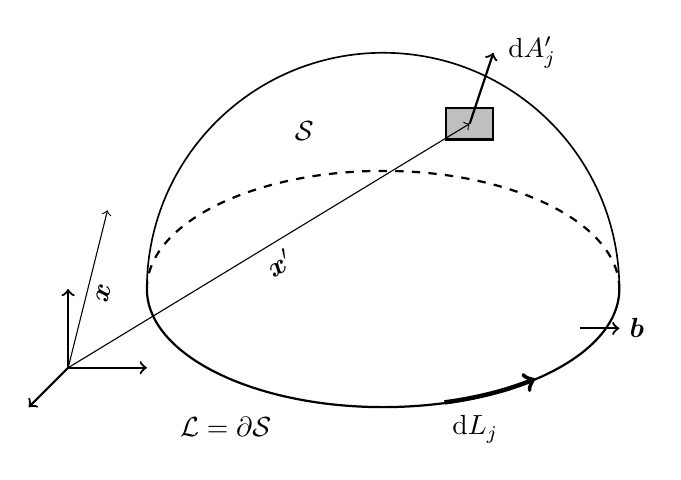
\begin{tikzpicture}
  \draw[semithick] (0,0) arc (0:180:3);
  \draw (-4,2) node {$\mathcal{S}$};
  \draw[dashed, thick] (0,0) arc [x radius=3, y radius=1.5, start angle=0, end angle=180];
  \draw[thick] (-6,0) arc [x radius=3, y radius=1.5, start angle=180, end angle=360];
  \draw[ultra thick, ->] (-2.22,-1.44) arc [x radius=3, y radius=1.5, start angle=285, end angle=310]
    node[below left, outer sep=10pt] {$\dL_j$};
  \filldraw[fill=gray!50!white, thick] (-2.2,2.3) rectangle (-1.6,1.9);
  \draw[thick, ->] (-1.9,2.1) -- (-1.6,3) node[right] {$\dA_j'$};
  \draw (-5,-1.5) node[below] {$\mathcal{L}=\partial\mathcal{S}$};
  \draw[->,thick] (-7,-1) -- (-7,-0); 
\draw[->,thick] (-7,-1) -- (-6,-1); 
\draw[->,thick] (-7,-1) -- (-7.5,-1.5); 
\draw[->] (-7,-1) --(-1.9,2.1)  node [sloped,below,text centered,midway]{$ \bm x'$}; 
\draw[->] (-7,-1) --(-6.5,1)  node [sloped,below,text centered,midway]{$ \bm x$}; 
\draw[->,thick] (-0.5,-0.5) --(-0,-0.5)  node [sloped,right,text centered]{$ \bm b$}; 
\end{tikzpicture}
\caption{The plastic distortion is concentrated on the surface $\mathcal{S}$, which is bounded by the dislocation line $\mathcal{L}=\partial\mathcal{S}$.}
\label{fig:dislocation_loop} 
\end{figure}
Let us know assume that the eigendistortion $\bm \beta^\star$ is only due to plastic deformation cause by dislocations, that is
\begin{align}
\bm \beta^\star=\bm \beta^P
\end{align}
The key equations of classical dislocation theory are now obtained by prescribing  the form of the eigendistortion tensor $\bm \beta^P$. For a dislocation extending over a surface $\mathcal{S}$,  the classical plastic eigendistortion tensor is taken in following form:
\begin{align}
\bPc_{kl}(\bm x)=-\int_\mathcal{S}\delta(\bm x-\bm x')b_k\dA_l'\, ,
\label{dislocation_distortion_classical}
\end{align}
where $\delta$ is the Dirac delta function, and $b_i$ is the displacement jump across $\mathcal{S}$, or Burgers vector. For a Volterra dislocation, as opposed to a Somigliana dislocation,  the Burgers vector is constant. In this case,  the  tensor $\alpha_{ij}=-\epsilon_{jkm}\bPc_{im,k}$ turns out to be concentrated on the dislocation line, that is the closed line $\mathcal{L}=\partial\mathcal{S}$ bounding the surface $\mathcal{S}$, and it is known as the \textit{dislocation density tensor}:
\begin{align}
\alpha_{ij}(\bm x)=\oint_{\mathcal{L}}\delta(\bm x-\bm x')b_i\dL_j'\, .
\label{dislocation_alpha_classical}
\end{align}
The rate of plastic distortion can be written in terms of the local dislocation velocity $w_k$ as
\begin{align}
\dot{\beta}^P_{ij}(\bm x)
=-\oint_{\mathcal{L}}\delta(\bm x-\bm x')b_i\epsilon_{jkm}w_k(\bm x')\dL_m'\,.
\label{plasticDistortionRateLoop}
\end{align}

Using the special forms (\ref{dislocation_distortion_classical}) and (\ref{dislocation_alpha_classical}) in the results obtained in the previous section we find all the key equations of classical dislocation theory in the anisotropic case. Letting $\bm R=\bm x-\bm x'$, these are:
\begin{subequations}
\begin{align}
u_i(\bm x)
&=-\frac{b_i\, \Omega(\bm
  x)}{4\pi}-\oint_{\mathcal{L}}\mathbb{C}_{mnpq}\epsilon_{jqr}b_pF_{jnim}(\bm
R)\dL_r' && \text{(anisotropic Burgers equation)}\\
\bEc_{ij}(\bm x)&=\oint_{\mathcal{L}}\mathbb{C}_{mnpq}\epsilon_{jqr}G_{im,n}(\bm R)b_p\dL_r' && \text{(Mura-Willis equation)}\\
\sigma_{ij}(\bm
x)&=\oint_{\mathcal{L}}\mathbb{C}_{ijkl}\mathbb{C}_{mnpq}\epsilon_{lqr}G_{km,n}(\bm
R)b_p\dL_r' && \text{(anisotropic Peach-Koehler stress equation)}\label{classicaCauchyStress}\\
W_{AB}&=\oint_{\mathcal{L}_A}\oint_{\mathcal{L}_B}\epsilon_{jkl}\mathbb{C}_{ilmn}\epsilon_{npq}\mathbb{C}_{rstp}F_{skmr}(\bm R)\, b^{A}_{t} b^{B}_{i} \dL^A_{q}\dL^B_{j}&&\text{(anisotropic Blin's formula) }\\
\mathcal{F}_k&=\oint_\mathcal{L}\epsilon_{kjm}\sigma_{ij}b_i\dL_m&&\text{(Peach-Koehler force)}
\end{align}
\label{class_aniso_all}
\end{subequations}
Note that, in the Burgers equation, we have introduced the solid angle  $\Omega(\bm x)$ subtended by the loop from the relationship  $\GP_{,j}*\bPc_{ij}=-{b_i\, \Omega}/{4\pi}$, which yields:
\begin{align}
\Omega(\bm x)=4\pi\int_\mathcal{S}\GP_{,j}\dA_j'=\int_\mathcal{S}\frac{R_j}{R^3}\dA_j'\, .
\end{align}

The kernel of Eq.~\eqref{}








%%%%%%%%%%%%%%%%%%%%%%%%%%%%%%%%%%%%%%%%%%
\section{The eigendistortion problem in the finite elastic medium: the superposition principle}

So far we have discussed the DDD method in the infinite elastic medium. However, many applications in micro-plasticity, such as micro indentation and micro-pillar compression, require that the dislocation network be embedded in a finite domain subject to prescribed boundary conditions. In order to extend the DDD method to finite domains, let us consider the eigenstrain problem in a finite domain   $\mathcal{B}$. In this case, the displacement field $u_k$ must satisfy the following boundary value problem (BVP) :
\begin{align}
\begin{cases}
\sigma_{ij}=c_{ijkl}\left(u_{k,l}-\beta^\star_{kl}\right) & \mbox{in }\mathcal{B}\\
\sigma_{ij,j}=0 & \mbox{in }\mathcal{B}\\
\sigma_{ij}\hat{n}_j=p_i & \mbox{on } \partial_N\mathcal{B}\\
u_i=\overline{u}_i & \mbox{on } \partial_D\mathcal{B}
\end{cases}
\label{BVPfinite}
\end{align}
where $p_i$ is the prescribed traction on the portion of the boundary $\partial_N\mathcal{B}$, and $\overline{u}_i$ is the prescribed displacement on the portion of the boundary $\partial_D\mathcal{B}$. Ideally, the BVP~(\ref{BVPfinite}) could be solved at each DDD step by incrementally updating $\beta^P_{ij}$ using its rate from eq.~(\ref{plasticDistortionRateLoop}). In a finite element framework this would provide the nodal displacements, from which the total stress could be computed and used to drive the discrete dislocation system inside $\mathcal{B}$. Practically, however, this approach is unfeasible because stresses, obtained as derivatives of displacement shape functions, would result in smooth fields which fail to  capture  sharp gradients in proximity of dislocation lines. In order to overcome this issue, an alternative formulation has been sought (c.f. \cite{eshelby1979boundary,Lubarda:1993uc,vanderGiessen:1995tm,Deng:2008fs,Weygand:2002tq}),  where the problem is decomposed into two auxiliary problems. The first problem, with infinite domain $\mathbb{R}^3$, consists in finding $u_i^\infty$ such that:
\begin{align}
\begin{cases}
\sigma^{\infty}_{ij}=c_{ijkl}(u^{\infty}_{k,l}-\beta^{P}_{kl}) & \mbox{in }\mathbb{R}^3\\
\sigma^{\infty}_{ij,j}=0 & \mbox{in }\mathbb{R}^3
\end{cases}
\label{BVPinfinite}
\end{align}
The second is a purely elastic ``correction" problem, with domain $\mathcal{B}$ consisting in finding $u_i^c$ such that:
\begin{align}
\begin{cases}
\sigma^c_{ij}=c_{ijkl}u^c_{k,l}& \mbox{in }\mathcal{B}\\
\sigma^c_{ij,j}=0 & \mbox{in }\mathcal{B}\\
\sigma^c_{ij}\hat{n}_j=p_i- \sigma^\infty_{ij}\hat{n}_j& \mbox{on } \partial_N\mathcal{B}\\
u_i^c=\overline{u}_i-u^\infty_i & \mbox{on } \partial_D\mathcal{B}
\end{cases}
\label{BVPcorrection}
\end{align}
The rationale behind this decomposition is clearly that (\ref{BVPinfinite}) is the standard dislocation eigenstrain problem in an infinite medium that we already solved in the previous sections. The total solution is clearly obtained as a sum: $u_i=u_i^\infty+u_i^c$ and the total stress field $\sigma_{ij}=\sigma_{ij}^\infty+\sigma_{ij}^c$ is used to drive dislocations in the finite-domain version of DDD.

%\begin{figure}[t]
%\centering\begin{tikzpicture}
%\draw [very thick] (-4,0) rectangle (4,3);
%\fill [fill=red!20!white] (-1.5,3.03) rectangle (1.5,5);
%\node at (0,4) {$\bm\beta^{P*}$};
%\node at (-3.5,0.5) {$\mathcal{B}$};
%  \begin{scope}[thick,decoration={
%    markings,
%    mark=at position 0.5 with {\arrow{>}}}
%    ] 
%    \draw[red!50!white,postaction={decorate}] (-1.5,5)--(1.5,5);
%    \draw[red!50!white,postaction={decorate}] (-1.5,3.03)--(-1.5,5);
%    \draw[red!50!white,postaction={decorate}] (1.5,5)--(1.5,3.03);
%    \draw[red!50!white,postaction={decorate}] (1.5,3.03)--(-1.5,3.03);
%\end{scope}
%\node at (0,5.2) {$\infty$};

% \begin{scope}[shift={(1.5,1)}]
%    \draw [blue,thick,domain=0:7.8540,variable=\t,smooth,samples=150]
%        plot ({\t r}: {0.032*\t*\t});
%  \end{scope}
%   \begin{scope}[shift={(-1.5,1)}]
%    \draw [blue,thick,domain=0:7.8540,variable=\t,smooth,samples=150]
%        plot ({-\t r}: {-0.032*\t*\t});
%  \end{scope}
  
%  \begin{scope}[thick,decoration={
%    markings,
%    mark=at position 0.5 with {\arrow{>}}}
%    ] 
%    \draw[blue,postaction={decorate}] (-1.5,2.97)--(1.5,2.97);
%\end{scope}
%\draw[->,thick] (2.5,1) --(3,0.5)  node [sloped,right,text centered]{\textcolor{black}{$ \bm b$}}; 
%\draw[->,thick] (1.25,4) --(1.75,3.5)  node [sloped,right,text centered]{\textcolor{black}{$ \bm b$}}; 
%\end{tikzpicture}
%\caption{Construction used for the solution of the BVP (\ref{BVPcorrection}). For each dislocation segment on the domain boundary a loop with the same Burgers vector and opposite line direction is constructed outside the integration domain, and encloses the virtual slip surface $\beta^{P*}$. One portion of the external loop coincides with the boundary segment, and the opposite side is pushed to infinity in the direction of the boundary normal.}
%\label{BVPStrategy}
%\end{figure}

From a numerical viewpoint, it is interesting to ask; what is the distribution of $\beta^P_{ij}$ outside $\mathcal{B}$ in (\ref{BVPinfinite})? We shall call this quantity $\beta^{P*}_{ij}$. In fact, although the solution to the problems (\ref{BVPinfinite}) and (\ref{BVPcorrection}) depend individually on $\beta^{P*}_{ij}$, it is easy to see that the total solution is independent of  $\beta^{P*}_{ij}$. Therefore $\beta^{P*}_{ij}$ can be chosen arbitrarily\footnote{We observe that the arbitrariness of $\beta^{P*}_{ij}$ implies that also its bounding curve (or virtual dislocation line) is arbitrary, in agreement with the ``mirror image construction" of \cite{Weygand:2002tq}  and the ``independence of the total stress on the choice of virtual segments'' mentioned in \cite{Weinberger:2009fk}.}.  The arbitrariness of $\beta^{P*}_{ij}$ can be exploited in the numerical implementation. To see how, we can cast  (\ref{BVPcorrection}) in its   corresponding Galerkin weak form
\begin{align}
\int_\mathcal{B}c_{ijkl}u^c_{k,l}\tilde{u}_{i,j}d\mathcal{V}=\int_{\partial_N\mathcal{B}}\left(p_i- \sigma^\infty_{ij}\hat{n}_j\right)\tilde{u}_id\mathcal{A}
\label{BVPcorrectionWeak}
\end{align} 
and notice that the RHS involves a surface integral  of the stress field  $\sigma^\infty_{ij}$ induced by the dislocation network. When a dislocation segment reaches the domain boundary, the numerical evaluation of this integral becomes challenging. This numerical difficulty can be  overcome using the construction shown in Fig.~\ref{BVPStrategy}. In fact, because $\beta^{P*}_{ij}$ is arbitrary, it is possible to add an external loop with the same Burgers vector of the boundary segment and opposite line direction, constructed so that one side of the loop overlaps with the boundary segment, and the opposite side is pushed to infinity along the direction of the boundary normal vector. In this way, because the contributions of the overlapping segments cancel out, the line integral involved in the calculation of $\sigma^{\infty}_{ij}$ can be limited to the portion of the dislocation configuration strictly inside the domain, and the virtual straight dislocation lines extending from the domain boundary to infinity. Notice that this construction unambiguously defines $\beta^{P*}_{ij}$ and the surface over which it extends, a fundamental requirement for the calculation of $u^\infty_i$ needed to satisfy displacement boundary conditions in the BVP (\ref{BVPcorrection}). 

\input{tex/MoDElib}

%%%%%%%%%%%%%%%%%%%%%%%%%
\appendix

\chapter{Review of tensor calculus}




\section{Mathematical preliminaries}

\subsection{Kelvin-Stokes Theorem}
\begin{mytheorem} (Kelvin-Stokes Theorem)
\begin{align}
\int_\mathcal{S} \epsilon_{ikl}f_{,l}\hat{n}_kds=\oint_{\partial\mathcal{S}} f dl_i
\label{KelvinStokes}
\end{align}
\end{mytheorem}

\begin{mytheorem} (Corollary)
\begin{align}
\int_\mathcal{S} \left(f_{,q}\hat{n}_p-f_{,p}\hat{n}_q\right)ds=\oint_{\partial\mathcal{S}} \epsilon_{ipq}f dl_i
\label{KelvinStokesCorollary}
\end{align}
\end{mytheorem}


%%%%%%%%%%%%%%%%%%%%%%%%%
\subsection{Surface Divergence Theorem}
In this section we recall some useful theorems in surface integration. \cite{Slattery2006}, \cite{Scovazzi2007}.

See \cite{Slattery:2006wn} p. 669.
\begin{mytheorem} (Surface Divergence Theorem)
fdsfsd
\end{mytheorem}

%%%%%%%%%%%%%%%%%%%%%%%%%
\subsection{Surface Transport Theorem}

\begin{mytheorem} (Surface Transport Theorem)
\begin{align}
\frac{d}{dt}\int_{\mathcal{S}_x=\bm \varphi (\mathcal{S}_X)}\alpha \hat{n}_ids&=\int_{\mathcal{S}_x}\left(\frac{\partial \alpha}{\partial t}+\left(\alpha \dot \varphi_k\right)_{,k}\right)\hat{n}_ids-\int_{\mathcal{S}_x}\alpha \dot\varphi_{k,i}\hat{n}_kds
\label{STT2}
\end{align}
\end{mytheorem}

\begin{proof}
From \cite{Scovazzi:2007tc}.
\end{proof}


\begin{mytheorem} (Surface Transport Theorem (alternative form))
\begin{align}
\frac{d}{dt}\int_{\mathcal{S}_x}\alpha ds&=\int_{\mathcal{S}_x}\frac{\partial \alpha}{\partial t}\hat{n}_ids+\oint\epsilon_{ikm}\alpha v_k dl_m+\int_{\mathcal{S}_x}\alpha_{,i} v_{k}\hat{n}_kds
\label{STT2L}
\end{align}
\end{mytheorem}

\begin{proof}
Consider the second term on the r.h.s. of~\ref{STT2} and use (\ref{KelvinStokesCorollary}):
\begin{align}
\int_{\mathcal{S}_x}\left(\alpha \dot \varphi_k\right)_{,k}\hat{n}_ids&=
\int_{\mathcal{S}_x}\left(\alpha \dot \varphi_k\right)_{,i}\hat{n}_kds+\oint\epsilon_{mik}\alpha v_k dl_m
\nonumber\\
\end{align}
Now consider the third term on the r.h.s. of~\ref{STT2} 
\begin{align}
\int_{\mathcal{S}_x}\alpha \dot\varphi_{k,i}\hat{n}_kds=\int_{\mathcal{S}_x}\left(\alpha v_{k}\right)_{,i}\hat{n}_kds-\int_{\mathcal{S}_x}\alpha_{,i} v_{k}\hat{n}_kds
\end{align}
Subtract to obtain result
\end{proof}


\begin{mytheorem} (Surface Transport Theorem (alternative form))
\begin{align}
\frac{d}{dt}\int_{\mathcal{S}_x=\bm \varphi (\mathcal{S}_X)}\alpha ds&=
\label{STT1}
\end{align}
\end{mytheorem}

\begin{proof}
See  \cite{Slattery:2006wn} p 61.
\end{proof}


%%%%%%%%%%%%%%%%%%%%%%
\subsection{Solid angles and line integration}

\begin{mytheorem} (Surface to Line integration)
Let $\mathcal{S}$ be a surface bounded by the closed contour $\Gamma$. Then let $\bm R=\bm R_s-\bm R_f$ where $\bm R_f$ is the field point and $\bm R_s$ is the source point on $\mathcal{S}$. If $\bm s$ is a unit vector applied at $\bm R_f$ such that the direction containing it never intersects $\mathcal{S}$ nor $\Gamma$, then: 
\begin{align}
-\int\frac{\bm R}{R^3} \cdot\hat{n}dS=\oint\frac{\bm s\times\bm R}{R(R-\bm s\cdot\bm R)}\cdot d\bm l
\label{solidAngle2Line}
\end{align}
Obviously if $\bm R$ has opposite definition, i.e. $\bm R=\bm R_f-\bm R_s$ then
\begin{align}
\int\frac{\bm R}{R^3} \cdot\hat{n}dS=-\oint\frac{\bm s\times\bm R}{R(R+\bm s\cdot\bm R)}\cdot d\bm l
\label{solidAngle2Line2}
\end{align}

\end{mytheorem}



Note that for unit vector $\bm s$ we have $\left(\bm R-R\bm s\right)^2=R^2+R^2-2R\bm R\cdot\bm s=2R(R-\bm R\cdot\bm s)$. This means that $2R(R-\bm R\cdot\bm s)=0$ only when $\bm R$ is aligned with $\bm s$.

\begin{proof}
From Stokes theorem:
\begin{align}
\oint\frac{\bm s\times\bm R}{R(R-\bm s\cdot\bm R)}\cdot d\bm l=\int\nabla\times\left[\frac{\bm s\times\bm R}{R(R-\bm s\cdot\bm R)}\right]ds
\end{align}
Now exapand the curl
\begin{align}
\nabla\times\left[\frac{\bm s\times\bm R}{R(R-\bm s\cdot\bm R)}\right]&=\epsilon_{ijk}\partial_j\left[\frac{\epsilon_{kmn}s_mR_n}{R(R-s_pR_p)}\right]=\left(\delta_{im}\delta_{jn}-\delta_{in}\delta_{jm}\right)\partial_j\left[\frac{s_mR_n}{R(R-s_pR_p)}\right]\nonumber\\
&=\left(\delta_{im}\delta_{jn}-\delta_{in}\delta_{jm}\right)\left[\frac{s_mR_{n,j}}{R(R-s_pR_p)}-\frac{s_mR_{n}\left[R_{,j}(R-s_pR_p)+R(R_{,j}-s_pR_{p,j})\right]}{R^2(R-s_pR_p)^2}\right]\nonumber\\
&=\left(\delta_{im}\delta_{jn}-\delta_{in}\delta_{jm}\right)\left[\frac{s_m\delta_{nj}}{R(R-s_pR_p)}-\frac{s_mR_{n}\left[\frac{R_j}{R}(R-s_pR_p)+R(\frac{R_j}{R}-s_p\delta_{pj})\right]}{R^2(R-s_pR_p)^2}\right]\nonumber\\
&=\left(\delta_{im}\delta_{jn}-\delta_{in}\delta_{jm}\right)\left[\frac{s_m\delta_{nj}}{R(R-s_pR_p)}-\frac{s_mR_{n}\left[\frac{R_j}{R}(R-s_pR_p)+(R_j-Rs_j)\right]}{R^2(R-s_pR_p)^2}\right]\nonumber\\
&=\left[\frac{\delta_{im}\delta_{jn}s_m\delta_{nj}}{R(R-s_pR_p)}-\frac{\delta_{im}\delta_{jn}s_mR_{n}\left[\frac{R_j}{R}(R-s_pR_p)+(R_j-Rs_j)\right]}{R^2(R-s_pR_p)^2}\right]\nonumber\\
&-\left[\frac{\delta_{in}\delta_{jm}s_m\delta_{nj}}{R(R-s_pR_p)}-\frac{\delta_{in}\delta_{jm}s_mR_{n}\left[\frac{R_j}{R}(R-s_pR_p)+(R_j-Rs_j)\right]}{R^2(R-s_pR_p)^2}\right]\nonumber\\
&=\left[\frac{3s_i}{R(R-s_pR_p)}-\frac{s_i\left[R(R-s_pR_p)+R(R-R_{j}s_j)\right]}{R^2(R-s_pR_p)^2}\right]\nonumber\\
&-\left[\frac{s_i}{R(R-s_pR_p)}-\frac{R_{i}\left[\frac{R_js_j}{R}(R-s_pR_p)+(R_js_j-R)\right]}{R^2(R-s_pR_p)^2}\right]\nonumber\\
&=\frac{3s_i}{R(R-s_pR_p)}-\frac{2s_i}{R(R-s_pR_p)}\nonumber\\
&-\frac{s_i}{R(R-s_pR_p)}+R_{i}\frac{\left[-R-\frac{R_js_js_pR_p}{R}+2R_js_j\right]}{R^2(R^2+s_pR_ps_jR_j-2Rs_pR_p)}\nonumber\\
&=-\frac{R_i}{R^3}
\end{align}
\end{proof}

   
   

%%%%%%%%%%%%%%%%%%%%%%%%%%%%%%%%%%%%%%%%%
\section{OLD NOTES: Elastic Energy of a Dislocation Loop}
\subsection{Volume to Surface}
(Eshelby) Let's consider a body delimited by a closed surface $S_0$ having a source of eigenstress\footnote{ no external surface traction}  $I$ enclosed within the surface $S$ and a source of stress $II$ outside $S$.

%and $V_I$ be a volume enclosing source $I$ then

\begin{eqnarray}
E&=&\frac{1}{2}\int_V\sigma_{ij}\epsilon_{ij}dV=\frac{1}{2}\int_V\left(\sigma^I_{ij}+\sigma^{II}_{ij}\right)\left(\epsilon^I_{ij}+\epsilon^{II}_{ij}\right)dV\nonumber\\
&=&\frac{1}{2}\int_V\sigma^I_{ij}\epsilon^{I}_{ij}dV+\frac{1}{2}\int_V\sigma^{II}_{ij}\epsilon^{II}_{ij}dV+\underbrace{\frac{1}{2}\int_V\sigma^{I}_{ij}\epsilon^{II}_{ij}dV+\frac{1}{2}\int_V\sigma^{II}_{ij}\epsilon^{I}_{ij}dV}_{\mbox{equal for reciprocity theorem}}\nonumber\\
&=&\underbrace{\frac{1}{2}\int_V\sigma^I_{ij}\epsilon^{I}_{ij}dV}_{E_I}+\underbrace{\frac{1}{2}\int_V\sigma^{II}_{ij}\epsilon^{II}_{ij}dV}_{E_{II}}+\underbrace{\int_V\sigma^{I}_{ij}\epsilon^{II}_{ij}dV}_{E_{int}}
\end{eqnarray}
Away from their respective sources strains are gradients of displacement fields therefore $\epsilon^{I}_{ij}=\frac{1}{2}\left(u^I_{i,j}+u^I_{j,i}\right)$ in $V_{II}$ and $\epsilon^{II}_{ij}=\frac{1}{2}\left(u^{II}_{i,j}+u^{II}_{j,i}\right)$ in $V_{I}$, but not conversely.
\begin{eqnarray}
E_{int}&=&\int_{V_I}\sigma^{I}_{ij}u^{II}_{i,j}dV_I+\int_{V_{II}}\sigma^{II}_{ij}u^{I}_{i,j}dV_{II}\noindent\\
&=&\oint_{S}\sigma^{I}_{ij}u^{II}_{i}\hat{n}_jdS-\underbrace{\int_{V_I}\sigma^{I}_{i,j}u^{II}_{i}dV_I}_{\mbox{equilibrium}}\nonumber\\
&+&\oint_{S_0}\sigma^{II}_{ij}u^{I}_{i}\hat{n}_jdS-\oint_{S}\sigma^{II}_{ij}u^{I}_{i}\hat{n}_jdS+\underbrace{\int_{V_{II}}\sigma^{II}_{i,j}u^{I}_{i}dV_{II}}_{\mbox{equilibrium}}\nonumber\\
&=&\oint_{S}\left(\sigma^{I}_{ij}u^{II}_{i}-\sigma^{II}_{ij}u^{I}_{i}\right)\hat{n}_jdS+\underbrace{\oint_{S_0}t_i^{II}u_i^{I}dS}_{\mbox{no surface tractions}}
\end{eqnarray}


the end result is

\begin{equation}
E_{int}=b_i\int_\mathcal{S} \sigma^{II}_{ij}\hat{n}_jdS
\end{equation}

%%%%%%%%%%%%%%%%%%%%%%%%%%%%%%%%%%

%\bibliographystyle{chicago} % authors sorted alphabetically
%\bibliography{references}

%\begin{thebibliography}{99}

%\bibitem{Slattery2006} Slattery, J. C., Sagis, L.,  Oh, E.-S. (2006). Interfacial Transport Phenomena, 2nd ed., Springer.

%
%\bibitem{Scovazzi2007} Scovazzi, G., Hughes, T. J. R. (2007). Lecture Notes on Continuum Mechanics on Arbitrary Moving Domains. cs.sandia.gov.






\section{Convolution integrals}
Throughout this document, the symbol $*$ stands for the convolution operator over the infinite three-dimensional space $\mathbb{R}^3$:
\begin{align}
f*g=\int_{\mathbb{R}^3}f(\bm x-\bm x')g(\bm x')\dV'
\end{align}
Convolution enjoys the following properties
\begin{align}
f*g=\int_{\mathbb{R}^3}f(\bm x-\bm x')g(\bm x')\dV'=-\int_{-\mathbb{R}^3}f(\bm x'')g(\bm x-\bm x'')\dV''=g*f
\end{align}

\begin{align}
(f*g)_{,i}=\int_{\mathbb{R}^3}f_{,i}(\bm x-\bm x')g(\bm x')\dV'=f_{,i}*g=f*g_{,i}
\end{align}

\begin{align}
(f*g)*h=f*(g*h)
\end{align}

\section{The nabla operator}


\section{The Green's  tensor and the F-tensor in classical  anisotropic elasticity}

\begin{figure}[t]
\centering
\include{fourierSphere}
%\includegraphics[width=0.4\textwidth]{fourierSphere}
\caption{The unit sphere in Fourier space. The unit vector $\bm \kappa(\theta,\phi)$ is defined by the azimuth angle $\phi$, and the  zenith angle $\theta$  measured from the axis $\hat{\bm e}_3=\bm R/R$.}
\label{kSpace}
\end{figure}

In classical  elasticity, the Green's  tensor of the anisotropic Navier operator $G^0_{ij}$ satisfies the following inhomogeneous PDE:
\begin{align}
L_{ik}G^0_{kj}+\delta_{ij}\delta=0\, .
\end{align}
In Fourier space\footnote{
The  Fourier transform  and its inverse are defined as, respectively ~\citep{Wl}:
\begin{align}
\hat{f}(\bm k)=\int_{\mathbb{R}^3} f(\bm x)\, \text{e}^{-\text{i}\bm k\cdot\bm x}\dV\,, &&
f(\bm x)=\frac{1}{(2\pi)^3}\int_{\mathbb{R}^3} \hat{f}(\bm k)\, \text{e}^{\text{i}\bm k\cdot\bm x}\, \text{d}\hat{V}\,.
\end{align}
} this reads:
\begin{align}
\hat{G}^0_{ik}(\bm k)=\frac{1}{k^2}\,\hat{L}^{-1}_{ik}(\bm \kappa)\, .
\end{align}
where $\hat{L}_{ik}(\bm \kappa)=\mathbb{C}_{ijkl}\kappa_j\kappa_l$, $\bm \kappa=\bm k/k$, and $k=\sqrt{\bm k\cdot\bm k}$. The Green's  tensor in real space  is obtained by inverse  Fourier transform. Expressing the elementary volume element in Fourier space as  $\text{d}\hat{V}=k^2\, \text{d}k\, \text{d}\omega$, where $\text{d}\omega$ is an elementary surface element of the unit sphere $\mathcal{S}$, we obtain:
\begin{align}
G^0_{ik}(\bm R)
&=\frac{1}{(2\pi)^3}\int_{\mathbb{R}^3} \frac{\hat{L}^{-1}_{ik}(\bm \kappa)}{k^2}\, \text{e}^{\text{i}\bm k\cdot\bm x} \, \text{d}\hat{V}
=\frac{1}{(2\pi)^3}\int_\mathcal{S}\hat{L}^{-1}_{kl}(\bm \kappa)\, \int_0^\infty \cos(k\bm\kappa\cdot\bm R)\, \text{d}k  \, \text{d}\omega\nonumber
=\frac{1}{8\pi^2R}\int_\mathcal{S}\hat{L}^{-1}_{kl}(\bm \kappa)\, \delta(\bm\kappa\cdot\bm R)  \, \text{d}\omega\, .
\end{align}
Choosing a reference system with $\hat{\bm e}_3$ aligned with $\bm R$, as shown in Fig.~\ref{kSpace}, and using the sifting property of the Dirac $\delta$-function, we finally obtain the expression for the Green tensor as:
\begin{align}
G^0_{ik}(\bm R)= \frac{1}{8\pi^2R}\int_0^{2\pi} \hat{L}^{-1}_{ik}(\bm n)\,  \text{d}\phi\,.
 \label{G0}
\end{align}
Here, $\bm n$ indicates a unit vector on the equatorial plane of the unit sphere in Fourier space. This result was first obtained by \cite{Lifshitz:1947aa} and \cite{Synge:1957aa}.

The classical $\bm F$-tensor, introduced by  \cite{Kirchner:1983}, is defined by Eq. \eqref{F_classical}, which in Fourier space reads:
\begin{align}
\hat{F}^0_{ijkl}=-\hat{G}^0_{kl}\,k_ik_j\,\hGP=-\frac{1}{k^2}\,\hat{L}^{-1}_{kl}(\bm \kappa)\,k_ik_j\, \frac{1}{k^2}=-\frac{1}{k^2}\,\hat{L}^{-1}_{kl}(\bm \kappa)\,\kappa_i\kappa_j\, .
\end{align}
The  classical $\bm F$-tensor in real space is obtained by inverse Fourier transform:
\begin{align}
F^0_{ijkl}(\bm R)&=-\frac{1}{(2\pi)^3}\int_{\mathbb{R}^3}\frac{1}{k^2}\,\hat{L}^{-1}_{kl}(\bm \kappa)\,\kappa_i\kappa_j\, \text{e}^{\text{i}\bm k\cdot\bm R} \, \text{d}\hat{V}
=-\frac{1}{(2\pi)^3}\int_\mathcal{S}\hat{L}^{-1}_{kl}(\bm \kappa)\,\kappa_i\kappa_j\,\, \int_0^\infty \cos(k\bm\kappa\cdot\bm R)\, \text{d}k  \, \text{d}\omega\nonumber\\
&=-\frac{1}{8\pi^2R}\int_\mathcal{S}\hat{L}^{-1}_{kl}(\bm \kappa)\,\kappa_i\kappa_j\, \delta(\bm\kappa\cdot\bm R)  \, \text{d}\omega\, .
\end{align}
In the reference system of Fig.~\ref{kSpace}, we finally obtain:
\begin{align}
F^0_{ijkl}(\bm R)&=-\frac{1}{8\pi^2R}\int_0^{2\pi}\hat{L}^{-1}_{kl}(\bm n)\,n_in_j\,   \, \text{d}\phi\, .
\label{F0}
\end{align}









\chapter{Elastic fields of piecewise-straight dislocations loop}



%%%%%%%%%%%%%%%%%%%%%%%%%
\subsection{Straight segments}
For a straight segment starting at $\bm A$ and ending at $\bm B$, it is useful to preliminary compute the function
\begin{align}
q(\bm x)=\int_{\bm A}^{\bm B}R_a\ d\ell'
\end{align}
where $R_a=\sqrt{\bm R\cdot\bm R+a^2}$, $\bm R=\bm x-\bm x'$. Integration is performed on the primed variable along the segment $\bm A\bm B$. This can be parametrized as a function of a scalar variable $u$ as
\begin{align}
\bm x'(u)=\bm A(1-u)+\bm Bu=\bm A+(\bm B-\bm A)u\hspace{1cm} u\in[0,1]
\end{align}
Therefore
\begin{align}
q(\bm x)&=L\int_0^1\sqrt{[(\bm A-\bm x)+(\bm B-\bm A)u]^2+a^2}\ du\nonumber\\
&=L\int_0^1\sqrt{(\bm B-\bm A)^2u^2+2(\bm A-\bm x)\cdot(\bm B-\bm A)u+(\bm A-\bm x)^2+a^2}\ du
\end{align}
Now
\begin{align}
\int\sqrt{du^2+bu+c}\ du=\left(\frac{b}{4d}+\frac{u}{2}\right)\sqrt{du^2+bu+c}+\frac{4dc-b^2}{8d^\frac{3}{2}}\ln\left(\frac{2du+b}{\sqrt{d}}+2\sqrt{du^2+bu+c}\right)
\end{align}
So
\begin{align}
\int_0^1\sqrt{du^2+bu+c}\ du=&\frac{2d+b}{4d}\sqrt{d+b+c}-\frac{b}{4d}\sqrt{c}+\frac{4dc-b^2}{8d^\frac{3}{2}}\ln\left(\frac{\frac{2d+b}{\sqrt{d}}+2\sqrt{d+b+c}}{\frac{b}{\sqrt{d}}+2\sqrt{c}}\right)
\end{align}

Note that in our case
\begin{align}
d&=(\bm B-\bm A)^2=L^2\\
b&=2(\bm A-\bm x)\cdot(\bm B-\bm A)=2L(\bm A-\bm x)\cdot\hat{\bm\xi}\\
c&=(\bm A-\bm x)^2+a^2\\
d+b+c&=(\bm B-\bm x)^2+a^2\\
2d+b&=2(\bm B-\bm x)\cdot(\bm B-\bm A)=2L(\bm B-\bm x)\cdot{\hat{\bm \xi}}\\
4dc-b^2&=4(\bm B-\bm A)^2(\bm A-\bm x)^2-[2(\bm A-\bm x)\cdot(\bm B-\bm A)]^2+4da^2\nonumber\\
&=4L^2[(\bm A-\bm x)^2-((\bm A-\bm x)\cdot\hat{\bm\xi})^2+a^2]\nonumber\\
&=4L^2[(\bm A-\bm B+\bm B-\bm x)^2-((\bm A-\bm x)\cdot\hat{\bm\xi})^2+a^2]\nonumber\\
&=4L^2[(\bm A-\bm B)^2+2(\bm A-\bm B)\cdot(\bm B-\bm x)+(\bm B-\bm x)^2-((\bm A-\bm B)\cdot\hat{\bm\xi}+(\bm B-\bm x)\cdot\hat{\bm\xi})^2+a^2]\nonumber\\
&=4L^2[L^2-2L\hat{\bm\xi}\cdot(\bm B-\bm x)+(\bm B-\bm x)^2-(-L+(\bm B-\bm x)\cdot\hat{\bm\xi})^2+a^2]\nonumber\\
&=4L^2[L^2-2L\hat{\bm\xi}\cdot(\bm B-\bm x)+(\bm B-\bm x)^2-L^2+2L(\bm B-\bm x)\cdot\hat{\bm\xi}-((\bm B-\bm x)\cdot\hat{\bm\xi})^2+a^2]\nonumber\\
&=4L^2[(\bm B-\bm x)^2-((\bm B-\bm x)\cdot\hat{\bm\xi})^2+a^2]\nonumber\\
&=4L^2\rho^2_a
\end{align}
where 
\begin{align}
\rho^2_a=(\bm B-\bm x)^2-((\bm B-\bm x)\cdot\hat{\bm\xi})^2+a^2=(\bm A-\bm x)^2-((\bm A-\bm x)\cdot\hat{\bm\xi})^2+a^2
\end{align}
$\rho^2$ is the regularized distance of $\bm x$ from the line passing through $\bm A$ and $\bm B$.

%\begin{align}
%\left(\frac{b}{4\, a} + \frac{1}{2}\right)\, \sqrt{a + b + c} - \left(\frac{b}{4\, a} - \frac{1}{2}\right)\, \sqrt{a - b + c} + \frac{\ln\!\left(\frac{a + \frac{b}{2}}{\sqrt{a}} + \sqrt{a + b + c}\right)\, \left(a\, c - \frac{b^2}{4}\right)}{2\, a^{\frac{3}{2}}} - \frac{\ln\!\left(\sqrt{a - b + c} - \frac{a - \frac{b}{2}}{\sqrt{a}}\right)\, \left(a\, c - \frac{b^2}{4}\right)}{2\, a^{\frac{3}{2}}}
%\end{align}


Therefore
\begin{align}
\int_0^1\sqrt{du^2+bu+c}\ du
%\frac{2a+b}{4a}\sqrt{a+b+c}-\frac{b}{4a}\sqrt{c}+\frac{4ac-b^2}{8a^\frac{3}{2}}\ln\left(\frac{\frac{2a+b}{\sqrt{a}}+2\sqrt{a+b+c}}{\frac{b}{\sqrt{a}}+2\sqrt{c}}\right)\nonumber\\
%&-\frac{4ac-b^2}{8a^\frac{3}{2}}\ln\left(\frac{b}{\sqrt{a}}+2\sqrt{c}\right)\nonumber\\
=&\frac{(\bm B-\bm x)\cdot(\bm B-\bm A)}{2(\bm B-\bm A)^2}\sqrt{(\bm B-\bm x)^2+a^2}-\frac{(\bm A-\bm x)\cdot(\bm B-\bm A)}{2(\bm B-\bm A)^2}\sqrt{(\bm A-\bm x)^2+a^2}\nonumber\\
&+\frac{4dc-b^2}{8L^3}\ln\left(\frac{\frac{2(\bm B-\bm x)\cdot(\bm B-\bm A)}{\sqrt{d}}+2\sqrt{(\bm B-\bm x)^2+a^2}}{\frac{2(\bm A-\bm x)\cdot(\bm B-\bm A)}{\sqrt{d}}+2\sqrt{(\bm A-\bm x)^2+a^2}}\right)\nonumber\\
=&\frac{(\bm B-\bm x)\cdot\hat{\bm\xi}}{2L}\sqrt{(\bm B-\bm x)^2+a^2}-\frac{(\bm A-\bm x)\cdot\hat{\bm\xi}}{2L}\sqrt{(\bm A-\bm x)^2+a^2}\nonumber\\
&+\frac{\rho^2_a}{2L}\ln\left(\frac{(\bm B-\bm x)\cdot\hat{\bm\xi}+\sqrt{(\bm B-\bm x)^2+a^2}}{(\bm A-\bm x)\cdot\hat{\bm\xi}+\sqrt{(\bm A-\bm x)^2+a^2}}\right)
\end{align}

If we define
\begin{align}
f(\bm z)
&=\frac{\bm z\cdot\hat{\bm\xi}}{2}z_a + \frac{\rho^2_a}{2}\ln\left(\bm z\cdot\hat{\bm\xi}+z_a\right)\nonumber\\
&=\frac{\bm z\cdot\hat{\bm\xi}}{2}z_a + \frac{\rho^2_a}{2}\ln\left(\bm Y_a\cdot\hat{\bm \xi}\right)
\end{align}
and
\begin{align}
\bm Y_a&=\bm z+z_a\hat{\bm\xi}\\
\rho_a^2&=\bm \rho_a\cdot\bm \rho_a=z^2-(\bm z\cdot\hat{\bm \xi})^2+a^2\\
\bm \rho_a&=\bm z-(\bm z\cdot\hat{\bm\xi}\pm a)\hat{\bm\xi}
\end{align}
then  we have
\begin{align}
q(\bm x)=f(\bm B-\bm x)-f(\bm A-\bm x)
\end{align}

Now consider the following identities:
\begin{align}
%\rho^2(\bm z)&=\bm \rho(\bm z)\cdot\bm \rho(\bm z)=z^2-(\bm z\cdot\hat{\bm \xi})^2\nonumber\\
\bm\rho_a\cdot\hat{\bm\xi}&=\mp a\\
%\rho_i{z}_i&=z^2-(\bm z\cdot\hat{\bm \xi})^2=\rho^2\\
\bm Y_a\cdot\hat{\bm \xi}&=\bm z\cdot\hat{\bm\xi}+z_a\\
Y^2_a&=2z_a\bm Y_a\cdot\hat{\bm \xi}-a^2\\
%\bm Y_a\cdot\bm z&=z(z+\bm z\cdot\hat{\bm\xi})=z\bm Y\cdot\hat{\bm \xi}\\
%\end{align}
%\begin{align}
\frac{\partial \rho_{ai}}{\partial z_j}&=\delta_{ij}-\hat{\xi}_i\hat{\xi}_j\\
%\end{align}
%\begin{align}
\frac{\partial \rho^2_a}{\partial z_i}&=2\rho_{ak} \frac{\partial  \rho_{ak}}{\partial z_i}=2\rho_{ak}\left(\delta_{ki}-\hat{\xi}_i\hat{\xi}_k\right)
%=2\left(\rho_i-\hat{\xi}_i\hat{\xi}_k\rho_k\right)\nonumber\\
%&=2\left[z_i-z_k\hat{\xi}_k\hat{\xi}_i-\hat{\xi}_i\left(z_m\hat{\xi}_m-z_k\hat{\xi}_k\hat{\xi}_m\hat{\xi}_m\right)\right]
=2(\underbrace{z_i-(\bm z\cdot\hat{\bm \xi})\hat{ \xi}_i}_{\rho_i})=2\rho_{i}\\
\frac{\partial \rho_{i}}{\partial z_j}&=\delta_{ij}-\hat{\xi}_i\hat{\xi}_j\\
%\end{align}
%\begin{align}
\frac{\partial Y_{ai}}{\partial z_j}&=\delta_{ij}+\frac{z_j\hat{\xi}_i}{z_a}\\
\frac{\partial (\bm Y_a \cdot \hat{\bm \xi})}{\partial z_i}&=\frac{ Y_{ai}}{z_a}\\
\frac{\partial }{\partial z_i}\ln (\bm Y_a \cdot \hat{\bm \xi})&=\frac{ Y_{ai}}{z_a \bm Y_a \cdot \hat{\bm \xi}}
\end{align}

First derivative
\begin{align}
\frac{\partial f}{\partial  z_i}
&=\frac{z_a\hat{\xi}_i}{2}+\frac{z_p\hat{\xi}_p z_i}{2z_a}+\rho_i\ln(\bm Y_a \cdot \hat{\bm \xi})+\frac{\rho^2_a}{2}\frac{ Y_{ai}}{z_a \bm Y_a \cdot \hat{\bm \xi}}\nonumber\\
&=\frac{z_a\hat{\xi}_i}{2}+\frac{z_p\hat{\xi}_p z_i}{2z_a}+\rho_i\ln(\bm Y_a \cdot \hat{\bm \xi})+\frac{(z^2-(z_q\hat{\xi}_q)^2+a^2)}{2}\frac{ Y_{ai}}{z_a (z_a+z_p\hat{\xi}_p)}\nonumber\\
&=\frac{z_a\hat{\xi}_i}{2}+\frac{z_p\hat{\xi}_p z_i}{2z_a}+\rho_i\ln(\bm Y_a \cdot \hat{\bm \xi})+\frac{(z_a-z_q\hat{\xi}_q)}{2}\frac{ Y_{ai}}{z_a }\nonumber\\
&=\frac{z_a^2\hat{\xi}_i+z_p\hat{\xi}_p z_i+(z_a-z_q\hat{\xi}_q)(z_i+z_a\hat{\xi}_i)}{2z_a}+\rho_i\ln(\bm Y_a \cdot \hat{\bm \xi})\nonumber\\
&=\frac{\rho_i}{2}+z_a\hat{\xi}_i+\rho_i\ln(\bm Y_a \cdot \hat{\bm \xi})
\end{align}


Second derivative
\begin{align}
\frac{\partial^2 f}{\partial  z_i\partial  z_j}
&=
\frac{\rho_{i,j}}{2}
+\frac{z_j}{z_a}\hat{\xi}_i
+ \rho_{i,j}\ln\left(\bm Y_a \cdot \hat{\bm \xi}\right)
+ \frac{\rho_iY_{aj}}{z_a \bm Y_a \cdot \hat{\bm \xi}}\nonumber\\
%
&=
\frac{ \delta_{ij}-\hat{\xi}_i\hat{\xi}_j}{2}
+\frac{z_j}{z_a}\hat{\xi}_i
+ (\delta_{ij}-\hat{\xi}_i\hat{\xi}_j)\ln\left(\bm Y_a \cdot \hat{\bm \xi}\right)
+ \frac{\rho_iY_{aj}}{z_a \bm Y_a \cdot \hat{\bm \xi}}\nonumber\\
&=
\frac{ \delta_{ij}-\hat{\xi}_i\hat{\xi}_j}{2}
+ (\delta_{ij}-\hat{\xi}_i\hat{\xi}_j)\ln\left(\bm Y_a \cdot \hat{\bm \xi}\right)
+ \frac{\rho_iY_{aj}+z_j\hat{\xi}_i \bm Y_a \cdot \hat{\bm \xi}}{z_a \bm Y_a \cdot \hat{\bm \xi}}
\nonumber\\
&=
\frac{ \delta_{ij}-\hat{\xi}_i\hat{\xi}_j}{2}
+ (\delta_{ij}-\hat{\xi}_i\hat{\xi}_j)\ln\left(\bm Y_a \cdot \hat{\bm \xi}\right)
+ \frac{1}{ \bm Y_a \cdot \hat{\bm \xi}}\left(\frac{z_iz_j}{z_a}+z_i\hat{\xi}_j+z_j\hat{\xi}_i-z_q\hat{\xi}_q\hat{\xi}_i\hat{\xi}_j\right)
\end{align}

\begin{align}
\frac{\partial^2 f}{\partial  z_p\partial  z_p}
&=1+ 2\ln\left(\bm Y_a \cdot \hat{\bm \xi}\right)+ \frac{1}{ \bm Y_a \cdot \hat{\bm \xi}}\left(\frac{z^2}{z_a}+\bm z\cdot\hat{\bm\xi}\right)\nonumber\\
&=1+ 2\ln\left(\bm Y_a \cdot \hat{\bm \xi}\right)+ \frac{1}{ \bm Y_a \cdot \hat{\bm \xi}}\left(z_a+\bm z\cdot\hat{\bm\xi}-\frac{a^2}{z_a}\right)\nonumber\\
&=2+ 2\ln\left(\bm Y_a \cdot \hat{\bm \xi}\right)-\frac{a^2}{z_a \bm Y_a \cdot \hat{\bm \xi}}
\label{laplacianFz}
\end{align}

Third derivative
\begin{align}
\frac{\partial^3 f}{\partial  z_i\partial  z_j z_m}
&=\frac{\delta_{jm}Y_{ai}+\delta_{im}Y_{aj}+\delta_{ij}Y_{am}}{z_a(\bm Y_a\cdot \hat{\bm \xi})}\\
&+\frac{1}{\bm Y_a\cdot \hat{\bm \xi}}\left(\frac{\bm z\cdot{\hat{\bm \xi}}}{\bm Y_a\cdot \hat{\bm \xi}}-2\right)\hat{\xi}_i\hat{\xi}_j\hat{\xi}_m\\
&-\frac{1}{z_a^2\bm Y_a\cdot \hat{\bm \xi}}\left(\frac{1}{\bm Y_a\cdot \hat{\bm \xi}}+\frac{1}{z_a}\right)z_iz_jz_m\\
&-\frac{\hat{\xi}_iz_mY_{aj}+\hat{\xi}_jz_iY_{am}+\hat{\xi}_mz_jY_{ai}}{z_a(\bm Y_a\cdot \hat{\bm \xi})^2}\\
\end{align}

Letting $i=j$
\begin{align}
\frac{\partial^3 f}{\partial  z_p\partial  z_p z_m}
&=\frac{5Y_{am}}{z_a(\bm Y_a\cdot \hat{\bm \xi})}\\
&+\frac{1}{\bm Y_a\cdot \hat{\bm \xi}}\left(\frac{\bm z\cdot{\hat{\bm \xi}}}{\bm Y_a\cdot \hat{\bm \xi}}+\frac{a^2}{z_a\bm Y_a\cdot \hat{\bm \xi}}-2\right)\hat{\xi}_m\\
&-\frac{1}{\bm Y_a\cdot \hat{\bm \xi}}\left(\frac{1}{\bm Y_a\cdot \hat{\bm \xi}}+\frac{1}{z_a}\right)\left(1-\frac{a^2}{z_a^2}\right)z_m\\
&-\frac{z_a+2(\bm z\cdot\hat{\bm \xi})}{z_a(\bm Y_a\cdot \hat{\bm \xi})^2}Y_{am}\nonumber\\
%
&=\frac{5Y_{am}}{z_a(\bm Y_a\cdot \hat{\bm \xi})}\\
&-\frac{z^2+z_a \bm Y_a\cdot \hat{\bm \xi}}{z_a(\bm Y_a\cdot \hat{\bm \xi})^2}\hat{\xi}_m\\
&-\frac{z_a+\bm Y_a\cdot \hat{\bm \xi}}{z_a(\bm Y_a\cdot \hat{\bm \xi})^2}\left(1-\frac{a^2}{z_a^2}\right)z_m\\
&-\frac{z_a+2(\bm z\cdot\hat{\bm \xi})}{z_a(\bm Y_a\cdot \hat{\bm \xi})^2}Y_{am}\\
%
&=\frac{5Y_{am}}{z_a(\bm Y_a\cdot \hat{\bm \xi})}\\
%&-\frac{z^2+z_a \bm Y_a\cdot \hat{\bm \xi}}{z_a(\bm Y_a\cdot \hat{\bm \xi})^2}\hat{\xi}_m\\
%&-\frac{z_a+\bm Y_a\cdot \hat{\bm \xi}}{z_a(\bm Y_a\cdot \hat{\bm \xi})^2}\left(1-\frac{a^2}{z_a^2}\right)z_m\\
&-\frac{z^2+z_a\bm Y_a\cdot \hat{\bm \xi}}{z_a^2(\bm Y_a\cdot \hat{\bm \xi})^2}Y_{am}+\frac{a^2}{z_a^3 \bm Y_a\cdot \hat{\bm \xi}}z_m\nonumber\\
&-\frac{z_a+2(\bm z\cdot\hat{\bm \xi})}{z_a(\bm Y_a\cdot \hat{\bm \xi})^2}Y_{am}\nonumber\\
%
&=\left(\frac{2}{z_a\bm Y_a\cdot \hat{\bm \xi}}+\frac{a^2}{z_a^2(\bm Y_a\cdot \hat{\bm \xi})^2}\right)Y_{am}+\frac{a^2}{z_a^3 \bm Y_a\cdot \hat{\bm \xi}}z_m
\end{align}



%Combining terms and using $\rho_m=Y_m-(\bm Y\cdot\hat{\bm \xi})\hat{\xi}_m$
%\begin{align}
%\frac{\partial^3 f}{\partial  z_p\partial  z_p z_m}
%&=\frac{1}{z(\bm Y\cdot \hat{\bm \xi})}\left(3-\frac{\bm z\cdot\hat{\bm\xi}}{(\bm Y\cdot \hat{\bm \xi})}\right)Y_m-\frac{1}{\bm Y\cdot \hat{\bm \xi}}\left(\frac{\rho_m}{\bm Y\cdot \hat{\bm \xi}}+\hat{\xi}_m\right)\nonumber\\
%&=\frac{2Y_m}{z\bm Y\cdot \hat{\bm \xi}}
%\end{align}

Since   $\epsilon_{klm}\hat{\xi}_l\hat{\xi}_m=0$, then $\epsilon_{klm}\hat{\xi}_lY_m=\epsilon_{klm}\hat{\xi}_lY_{am}=\epsilon_{klm}\hat{\xi}_l\rho_m=\epsilon_{klm}\hat{\xi}_lz_m$. Therefore 
\begin{align}
\epsilon_{klm}\hat{\xi}_l\frac{\partial^3 f}{\partial  z_i\partial  z_j z_m}
&=\frac{\epsilon_{klj}\hat{\xi}_lY_{ai}+\epsilon_{kli}\hat{\xi}_lY_{aj}+\epsilon_{klm}\hat{\xi}_l\delta_{ij}Y_{am}}{z_a(\bm Y_a\cdot \hat{\bm \xi})}\\
&-\epsilon_{klm}\hat{\xi}_l\frac{1}{z_a^2\bm Y_a\cdot \hat{\bm \xi}}\left(\frac{1}{\bm Y_a\cdot \hat{\bm \xi}}+\frac{1}{z_a}\right)z_iz_jY_{am}\\
&-\frac{\epsilon_{klm}\hat{\xi}_l\hat{\xi}_iY_{am}Y_{aj}+\epsilon_{klm}\hat{\xi}_l\hat{\xi}_jz_iY_{am}}{z_a(\bm Y_a\cdot \hat{\bm \xi})^2}
\end{align}
and
\begin{align}
\epsilon_{klm}\hat{\xi}_l\frac{\partial^3 f}{\partial  z_p\partial  z_p z_m}&=\epsilon_{klm}\hat{\xi}_l\left(\frac{2}{z_a\bm Y_a\cdot \hat{\bm \xi}}+\frac{a^2}{z_a^2(\bm Y_a\cdot \hat{\bm \xi})^2}+\frac{a^2}{z_a^3 \bm Y_a\cdot \hat{\bm \xi}}\right)Y_{am}
\end{align}

Simplifying:
\begin{align}
\epsilon_{klm}\hat{\xi}_l\frac{\partial^3 f}{\partial  z_i\partial  z_j z_m}&=
\frac{\epsilon_{klj}\hat{\xi}_lY_{ai}+\epsilon_{kli}\hat{\xi}_lY_{aj}}{z_a(\bm Y_a\cdot \hat{\bm \xi})}\nonumber\\
&+\frac{\epsilon_{klm}\hat{\xi}_lY_{am}}{z_a(\bm Y_a\cdot \hat{\bm \xi})}\left[\delta_{ij}-\frac{z_a+\bm Y_a\cdot \hat{\bm \xi}}{z_a^2\bm Y_a\cdot \hat{\bm \xi}}z_iz_j-\frac{\hat{\xi}_iz_j+\hat{\xi}_jz_i+z_a\hat{\xi}_i\hat{\xi}_j}{\bm Y_a\cdot \hat{\bm \xi}}\right]\\
\end{align}


 
%%%%%%%%%%%%%%%%%%%%%%%%%
\subsection{Stress field of a straight segment}


The stress field of the segment $\bm A\rightarrow\bm B$ is
\begin{align}
\sigma_{ij}(\bm x)=b_k\int_{\bm A}^{\bm B}S_{ijkl}R_a\ d\ell'_l
\end{align}
\begin{align}
S_{ijkl}=\frac{\mu}{8\pi}\left[\left(\delta_{il}\epsilon_{jmk}+\delta_{jl}\epsilon_{imk}\right)\partial_m\Delta+\frac{2}{1-\nu}\epsilon_{klm}\left(\partial_{i}\partial_j\partial_m-\delta_{ij}\partial_m\Delta\right)\right]
\end{align}
Now notice that differentiation is in $\bm x$, while integration is in $\bm x'$. Therefore they commute. 
\begin{align}
\sigma_{ij}(\bm x)
&=b_k\hat{\xi}_lS_{ijkl}q(\bm x)\nonumber\\
&=\hat{\xi}_lb_k\frac{\mu}{8\pi}\left[\left(\delta_{il}\epsilon_{jmk}+\delta_{jl}\epsilon_{imk}\right)\partial_m\Delta+\frac{2}{1-\nu}\epsilon_{klm}\left(\partial_{i}\partial_j\partial_m-\delta_{ij}\partial_m\Delta\right)\right]\left[f(\bm B-\bm x)-f(\bm A-\bm x)\right]\nonumber\\
&=\hat{\xi}_lb_k\frac{\mu}{8\pi}\left[\left(\delta_{il}\epsilon_{jmk}+\delta_{jl}\epsilon_{imk}\right)\partial_m\Delta+\frac{2}{1-\nu}\epsilon_{klm}\left(\partial_{i}\partial_j\partial_m-\delta_{ij}\partial_m\Delta\right)\right]\left[f(\bm z)\right]^{\bm z=\bm B-\bm x}_{\bm z=\bm A-\bm x}\nonumber\\
&=\frac{\mu}{4\pi(1-\nu)}\left[\frac{1-\nu}{2}\left(\hat{\xi}_ib_k\epsilon_{jmk}+\hat{\xi}_jb_k\epsilon_{imk}\right)\frac{\partial^3 f}{\partial z_p\partial z_p\partial z_m}+\epsilon_{klm}\hat{\xi}_lb_k\left(\frac{\partial^3 f}{\partial z_i\partial z_j\partial z_m}-\delta_{ij}\frac{\partial^3 f}{\partial z_p\partial z_p\partial z_m}\right)\right]^{\bm z=\bm A-\bm x}_{\bm z=\bm B-\bm x}
\label{stressStraightDerivation}
\end{align}
 
Plugging back in \eqref{stressStraightDerivation} we obtain
\begin{align}
\sigma_{ij}(\bm x)
=\frac{\mu}{4\pi(1-\nu)}&\left[\frac{1-\nu}{2}\left(\hat{\xi}_ib_k\epsilon_{jmk}+\hat{\xi}_jb_k\epsilon_{imk}\right)\left[\left(\frac{2}{z_a\bm Y_a\cdot \hat{\bm \xi}}+\frac{a^2}{z_a^2(\bm Y_a\cdot \hat{\bm \xi})^2}\right)Y_{am}+\frac{a^2}{z_a^3 \bm Y_a\cdot \hat{\bm \xi}}z_m\right]\right.\nonumber\\
&+\frac{\epsilon_{klj}b_k\hat{\xi}_lY_{ai}+\epsilon_{kli}b_k\hat{\xi}_lY_{aj}}{z_a(\bm Y_a\cdot \hat{\bm \xi})}\nonumber\\
&+\frac{\epsilon_{klm}b_k\hat{\xi}_lY_{am}}{z_a(\bm Y_a\cdot \hat{\bm \xi})}\left(\delta_{ij}-\frac{z_a+\bm Y_a\cdot \hat{\bm \xi}}{z_a^2\bm Y_a\cdot \hat{\bm \xi}}z_iz_j-\frac{\hat{\xi}_iz_j+\hat{\xi}_jz_i+z_a\hat{\xi}_i\hat{\xi}_j}{\bm Y_a\cdot \hat{\bm \xi}}\right)\nonumber\\
&\left.-\epsilon_{klm}b_k\hat{\xi}_lY_{am}\delta_{ij}\left(\frac{2}{z_a\bm Y_a\cdot \hat{\bm \xi}}+\frac{a^2}{z_a^2(\bm Y_a\cdot \hat{\bm \xi})^2}+\frac{a^2}{z_a^3 \bm Y_a\cdot \hat{\bm \xi}}\right)\right]^{\bm z=\bm A-\bm x}_{\bm z=\bm B-\bm x}
\end{align}
Factoring the term $z_a\bm Y_a\cdot \hat{\bm \xi}=(Y_a^2+a^2)/2$ we obtain
\begin{align}
\sigma_{ij}(\bm x)
=\frac{\mu}{4\pi(1-\nu)}&\left[\frac{2}{Y_a^2+a^2}\left\{(1-\nu)\left(\hat{\xi}_ib_k\epsilon_{jmk}+\hat{\xi}_jb_k\epsilon_{imk}\right)\left[\left(1+\frac{a^2}{Y_a^2+a^2}\right)Y_{am}+\frac{a^2}{2z_a^2 }z_m\right]\right.\right.\nonumber\\
&+\epsilon_{klj}b_k\hat{\xi}_lY_{ai}+\epsilon_{kli}b_k\hat{\xi}_lY_{aj}\nonumber\\
&\left.\left.-\epsilon_{klm}b_k\hat{\xi}_lY_{am}\left(\left(1+2\frac{a^2}{Y_a^2+a^2}+\frac{a^2}{z_a^2 }\right)\delta_{ij}+2\frac{z_a+\bm Y_a\cdot \hat{\bm \xi}}{z_a(Y_a^2+a^2)}z_iz_j+\frac{\hat{\xi}_iz_j+\hat{\xi}_jz_i+z_a\hat{\xi}_i\hat{\xi}_j}{\bm Y_a\cdot \hat{\bm \xi}}\right)
\right\}\right]^{\bm z=\bm A-\bm x}_{\bm z=\bm B-\bm x}
%\nonumber\\
%
%&\left.\left.-\epsilon_{klm}b_k\hat{\xi}_lY_{am}\delta_{ij}\left(2+\frac{a^2}{z_a\bm Y_a\cdot \hat{\bm \xi}}+\frac{a^2}{z_a^2 }\right)\right\}\right]^{\bm z=\bm A-\bm x}_{\bm z=\bm B-\bm x}
\end{align}


%\begin{align}
%\sigma_{ij}(\bm x)
%=\frac{\mu}{4\pi(1-\nu)}&\left[\frac{2}{Y^2}\left\{(1-\nu)\left(\hat{\xi}_i\epsilon_{jmk}Y_mb_k+\epsilon_{imk}Y_mb_k\hat{\xi}_j\right)\right.\right.\nonumber\\
%&+Y_i\epsilon_{jkl}b_k\hat{\xi}_l+\epsilon_{ikl}b_k\hat{\xi}_lY_j\nonumber\\
%&\left.\left.-\epsilon_{klm}b_k\hat{\xi}_lY_m\left(\delta_{ij}+2\frac{z+\bm Y\cdot \hat{\bm \xi}}{zY^2}z_iz_j+\frac{\hat{\xi}_iz_j+\hat{\xi}_jz_i+z\hat{\xi}_i\hat{\xi}_j}{\bm Y\cdot \hat{\bm \xi}}\right)\right\}\right]^{\bm z=\bm A-\bm x}_{\bm z=\bm B-\bm x}
%&\left.\left.-\epsilon_{klm}\hat{\xi}_lb_k\delta_{ij}\frac{2Y_m}{Y^2}\right\}\right]^{\bm z=\bm A-\bm x}_{\bm z=\bm B-\bm x}
%\end{align}
Inverting the order of evaluation, and changing the sign within the square bracket we have
\begin{align}
\sigma_{ij}(\bm x)
=\frac{\mu}{4\pi(1-\nu)}&\left[\frac{2}{Y_a^2+a^2}\left\{(1-\nu)\left(\hat{\xi}_ib_k\epsilon_{jkm}+\hat{\xi}_jb_k\epsilon_{ikm}\right)\left[\left(1+\frac{a^2}{Y_a^2+a^2}\right)Y_{am}+\frac{a^2}{2z_a^2 }z_m\right]\right.\right.\nonumber\\
&-(Y_{ai}\epsilon_{jkl}b_k\hat{\xi}_l+\epsilon_{ikl}b_k\hat{\xi}_lY_{aj})\nonumber\\
&\left.\left.-\epsilon_{klm}b_kY_{al}\hat{\xi}_m\left(\left(1+2\frac{a^2}{Y_a^2+a^2}+\frac{a^2}{z_a^2 }\right)\delta_{ij}+2\frac{z_a+\bm Y_a\cdot \hat{\bm \xi}}{z_a(Y_a^2+a^2)}z_iz_j+\frac{\hat{\xi}_iz_j+\hat{\xi}_jz_i+z_a\hat{\xi}_i\hat{\xi}_j}{\bm Y_a\cdot \hat{\bm \xi}}\right)
\right\}\right]^{\bm z=\bm B-\bm x}_{\bm z=\bm A-\bm x}
%\nonumber\\
%
%&\left.\left.-\epsilon_{klm}b_k\hat{\xi}_lY_{am}\delta_{ij}\left(2+\frac{a^2}{z_a\bm Y_a\cdot \hat{\bm \xi}}+\frac{a^2}{z_a^2 }\right)\right\}\right]^{\bm z=\bm A-\bm x}_{\bm z=\bm B-\bm x}
\end{align}

%\begin{align}
%\sigma_{ij}(\bm x)
%=\frac{\mu}{4\pi(1-\nu)}&\left[\frac{2}{Y^2}\left\{(1-\nu)\left(\hat{\xi}_i\epsilon_{jkm}b_kY_m+\epsilon_{ikm}b_kY_m\hat{\xi}_j\right)\right.\right.\nonumber\\
%&-\left(Y_i\epsilon_{jkl}b_k\hat{\xi}_l+\epsilon_{ikl}b_k\hat{\xi}_lY_j\right)\nonumber\\
%&\left.\left.-\epsilon_{klm}b_kY_l\hat{\xi}_m\left(\delta_{ij}+2\frac{z+\bm Y\cdot \hat{\bm \xi}}{zY^2}z_iz_j+\frac{\hat{\xi}_iz_j+\hat{\xi}_jz_i+z\hat{\xi}_i\hat{\xi}_j}{\bm Y\cdot \hat{\bm \xi}}\right)\right\}\right]^{\bm z=\bm B-\bm x}_{\bm z=\bm A-\bm x}
%&\left.\left.-\epsilon_{klm}\hat{\xi}_lb_k\delta_{ij}\frac{2Y_m}{Y^2}\right\}\right]^{\bm z=\bm A-\bm x}_{\bm z=\bm B-\bm x}
%\end{align}
It is more efficient to compute the stress field as
\begin{align}
\bm\sigma(\bm x)=\frac{\mu}{4\pi(1-\nu)}\left(\bm s(\bm x)+\bm s^T(\bm x)\right)
\end{align}
where
\begin{align}
\bm s(\bm x)=\tilde {\bm s}(\bm B-\bm x)-\tilde {\bm s}(\bm A-\bm x)
\end{align}
and
\begin{align}
\tilde{\bm s}(\bm z)
=\frac{2}{Y_a^2+a^2}&
\left\{
(1-\nu)\left(1+\frac{a^2}{Y_a^2+a^2}\right)\hat{\bm\xi}\otimes\left(\bm b\times \bm Y_a\right)\right.\nonumber\\
&+(1-\nu)\frac{a^2}{2z_a^2 }\hat{\bm\xi}\otimes\left(\bm b\times \bm z\right)\nonumber\\
&-\bm Y_a\otimes\left(\bm b\times\hat{\bm \xi}\right)\nonumber\\
&-\frac{\left[\left(\bm b\times\bm Y_a\right)\cdot\hat{\bm \xi}\right]}{\bm Y_a\cdot \hat{\bm \xi}}\hat{\bm\xi}\otimes\bm z\nonumber\\
&\left.-\frac{\left[\left(\bm b\times\bm Y_a\right)\cdot\hat{\bm \xi}\right]}{2}\left(\left(1+2\frac{a^2}{Y_a^2+a^2}+\frac{a^2}{z_a^2 }\right)\bm I+2\frac{z_a+\bm Y_a\cdot \hat{\bm \xi}}{z_a(Y_a^2+a^2)}\bm z\otimes\bm z+\frac{z_a}{\bm Y_a\cdot \hat{\bm \xi}}\hat{\bm\xi}\otimes\hat{\bm\xi}\right)\right\}%\right]^{\bm z=\bm B-\bm x}_{\bm z=\bm A-\bm x}
%&\left.\left.-\epsilon_{klm}\hat{\xi}_lb_k\delta_{ij}\frac{2Y_m}{Y^2}\right\}\right]^{\bm z=\bm A-\bm x}_{\bm z=\bm B-\bm x}
\end{align}
with
\begin{align}
\bm Y_a(\bm z)&=\bm z+z_a\hat{\bm\xi}\\
 Y^2_a(\bm z)&=2z_a\bm Y_a\cdot\hat{\bm \xi}-a^2
 %=z^2+2z_a\bm z\cdot\hat{\bm\xi}+z_a^2\\
\end{align}
Note that
\begin{align}
\left( Y^2_a+a^2\right)^2&=4z_a^2\left(\bm Y_a\cdot\hat{\bm \xi}\right)^2=4z_a^2\left(\bm z\cdot\hat{\bm \xi}+z_a\right)^2
 %=z^2+2z_a\bm z\cdot\hat{\bm\xi}+z_a^2\\
\end{align}

\subsubsection{Stress of a straight segment on a distant point}
Suppose that we want to compute the stress field of a segment $\bm A\bm B$ at a point $\bm x$, which is located at distance $d$ from the center $\bm C$ of the segment. Let the length of the segment be $AB=2L$, then
\begin{align}
\bm B-\bm x&=\bm C-\bm x+\bm C-\bm B=\bm C-\bm x-L\hat{\bm\xi}=d\left(\hat{\bm r}_c-\frac{L}{d}\hat{\bm\xi}\right)\\
\bm A-\bm x&=\bm C-\bm x+\bm C-\bm A=\bm C-\bm x+L\hat{\bm\xi}=d\left(\hat{\bm r}_c+\frac{L}{d}\hat{\bm\xi}\right)
\end{align}
where $\hat{\bm r}_c=(\bm C-\bm x)/\|\bm C-\bm x\|=(\bm C-\bm x)/d$. Therefore we have
\begin{align}
\bm s(\bm x)=\tilde {\bm s}\left(d\left(\hat{\bm r}_c-\frac{L}{d}\hat{\bm\xi}\right)\right)-
\tilde {\bm s}\left(d\left(\hat{\bm r}_c+\frac{L}{d}\hat{\bm\xi}\right)\right)
%\tilde {\bm s}(\bm A-\bm x)
\end{align}
%\begin{align}
%\bm s(\bm x)
%=\left[\frac{2}{Y^2}\right.&
%\left\{
%(1-\nu)\hat{\bm\xi}\otimes\left(\bm b\times \bm Y\right)\right.\nonumber\\
%&-\bm Y\otimes\left(\bm b\times\hat{\bm \xi}\right)\nonumber\\
%&-\frac{\left[\left(\bm b\times\bm Y\right)\cdot\hat{\bm \xi}\right]}{\bm Y\cdot \hat{\bm \xi}}\hat{\bm\xi}\otimes\bm z\nonumber\\
%&\left.\left.-\frac{\left[\left(\bm b\times\bm Y\right)\cdot\hat{\bm \xi}\right]}{2}\left(\bm I+2\frac{z+\bm Y\cdot \hat{\bm \xi}}{zY^2}\bm z\otimes\bm z+\frac{z}{\bm Y\cdot \hat{\bm \xi}}\hat{\bm\xi}\otimes\hat{\bm\xi}\right)\right\}\right]^{\bm z=d\left(\hat{\bm r}_c-\frac{L}{d}\hat{\bm\xi}\right)}_{\bm z=d\left(\hat{\bm r}_c+\frac{L}{d}\hat{\bm\xi}\right)}
%\end{align}
If $d$ is large compared to the segment length, that is 
\begin{align}
\frac{L}{d}\ll1
\end{align}
then the difference above can be approximated  as
\begin{align}
\bm s(\bm x)\approx \left.\frac{\partial \tilde {\bm s}(\bm z)}{\partial \bm z}\right|_{\bm z=\bm C-\bm x}\cdot(-2L\hat{\bm \xi})
%\left(d\left(\hat{\bm r}_c-\frac{L}{d}\hat{\bm\xi}\right)\right)-
%\tilde {\bm s}\left(d\left(\hat{\bm r}_c+\frac{L}{d}\hat{\bm\xi}\right)\right)
%\tilde {\bm s}(\bm A-\bm x)
\end{align}
Note that 
\begin{align}
\frac{\partial {Y_i}}{\partial z_j}\hat{\xi}_j=\frac{\bm Y\cdot\hat{\bm\xi}}{z}\hat{\xi}_i
\end{align}
then
\begin{align}
\frac{\partial \tilde {\bm s}(\bm z)}{\partial \bm z}
=\frac{\partial}{\partial \bm z}\left[\frac{2}{Y^2}\right.&
\left\{
(1-\nu)\hat{\bm\xi}\otimes\left(\bm b\times \bm Y\right)\right.\nonumber\\
&-\bm Y\otimes\left(\bm b\times\hat{\bm \xi}\right)\nonumber\\
&-\frac{\left[\left(\bm b\times\bm Y\right)\cdot\hat{\bm \xi}\right]}{\bm Y\cdot \hat{\bm \xi}}\hat{\bm\xi}\otimes\bm z\nonumber\\
&\left.\left.-\frac{\left[\left(\bm b\times\bm Y\right)\cdot\hat{\bm \xi}\right]}{2}\left(\bm I+2\frac{z+\bm Y\cdot \hat{\bm \xi}}{zY^2}\bm z\otimes\bm z+\frac{z}{\bm Y\cdot \hat{\bm \xi}}\hat{\bm\xi}\otimes\hat{\bm\xi}\right)\right\}\right]\cdot(-2L\hat{\bm \xi})\nonumber\\
%
&=\left[-\frac{2}{Y}\frac{\partial Y}{\partial \bm z}\cdot\left(-2L\hat{\bm \xi}\right)\right]\tilde{\bm s}(\bm z)\nonumber\\
&+\frac{2}{Y^2}\left[\frac{\partial}{\partial \bm z}
\left\{
(1-\nu)\hat{\bm\xi}\otimes\left(\bm b\times \bm Y\right)\right.\right.\nonumber\\
&-\bm Y\otimes\left(\bm b\times\hat{\bm \xi}\right)\nonumber\\
&-\frac{\left[\left(\bm b\times\bm Y\right)\cdot\hat{\bm \xi}\right]}{\bm Y\cdot \hat{\bm \xi}}\hat{\bm\xi}\otimes\bm z\nonumber\\
&\left.\left.-\frac{\left[\left(\bm b\times\bm Y\right)\cdot\hat{\bm \xi}\right]}{2}\left(\bm I+2\frac{z+\bm Y\cdot \hat{\bm \xi}}{zY^2}\bm z\otimes\bm z+\frac{z}{\bm Y\cdot \hat{\bm \xi}}\hat{\bm\xi}\otimes\hat{\bm\xi}\right)\right\}\right]\cdot(-2L\hat{\bm \xi})\nonumber\\
%
&=\frac{4L}{zY^2}\left(\bm Y\cdot\hat{\bm \xi}\right)^2\tilde{\bm s}(\bm z)\nonumber\\
&-\frac{4L}{Y^2}\left[
\left\{
(1-\nu)\frac{\bm Y\cdot\hat{\bm \xi}}{z}\hat{\bm\xi}\otimes\left(\bm b\times \hat{\bm \xi}\right)\right.\right.\nonumber\\
&-\frac{\bm Y\cdot\hat{\bm \xi}}{z}\hat{\bm \xi}\otimes\left(\bm b\times\hat{\bm \xi}\right)\nonumber\\
&+\frac{\left[\left(\bm b\times\bm Y\right)\cdot\hat{\bm \xi}\right]}{z\bm Y\cdot \hat{\bm \xi}}\hat{\bm\xi}\otimes\bm z
-\frac{\left[\left(\bm b\times\bm Y\right)\cdot\hat{\bm \xi}\right]}{\bm Y\cdot \hat{\bm \xi}}\hat{\bm\xi}\otimes\hat{\bm \xi}\nonumber\\
&\left.\left.-\left[\left(\bm b\times\bm Y\right)\cdot\hat{\bm \xi}\right]\left(\frac{z+\bm Y\cdot \hat{\bm \xi}}{zY^2}\bm z\otimes\bm z\right)\cdot\hat{\bm \xi}\right\}\right]\nonumber\\
&\left.\left.-\frac{\left[\left(\bm b\times\bm Y\right)\cdot\hat{\bm \xi}\right]}{2}\frac{\partial}{\partial \bm z}\left(\frac{z}{\bm Y\cdot \hat{\bm \xi}}\hat{\bm\xi}\otimes\hat{\bm\xi}\right)\cdot\hat{\bm \xi}\right\}\right]\nonumber\\
\end{align}

Now let $C$ be the center of the segment $\bm A\bm B$, so that  


\subsubsection{Stress of a straight segment in the neighborhood of a far point}

Suppose that we want to compute the stress field of segment $\bm A\bm B$ at a point $\bm x$ which is in the neighborhood of a point $\bm x_0$. Let the distance from $\bm x_0$ to the segment $\bm A\bm B$ be $d$. Then we work under the assumption $AB\ll d$ and $\|\bm x-\bm x_0\|\ll d$. 


%\begin{align}
%\bm s(\bm x)
%=&\left[\frac{2}{Y^2}\left\{(1-\nu)\hat{\bm\xi}\otimes\left(\bm b\times \bm Y\right)\right.\right.\nonumber\\
%&-\bm Y\otimes\left(\bm b\times\hat{\bm \xi}\right)\nonumber\\
%&-\frac{\left[\left(\bm b\times\bm Y\right)\cdot\hat{\bm \xi}\right]}{\bm Y\cdot \hat{\bm \xi}}\hat{\bm\xi}\otimes\bm z\nonumber\\
%&\left.\left.-\frac{\left[\left(\bm b\times\bm Y\right)\cdot\hat{\bm \xi}\right]}{2}\left(\bm I+2\frac{z+\bm Y\cdot \hat{\bm \xi}}{zY^2}\bm z\otimes\bm z+\frac{z\hat{\xi}_i\hat{\xi}_j}{\bm Y\cdot \hat{\bm \xi}}\right)\right\}\right]^{\bm z=\bm B-\bm x}_{\bm z=\bm A-\bm x}
%&\left.\left.-\epsilon_{klm}\hat{\xi}_lb_k\delta_{ij}\frac{2Y_m}{Y^2}\right\}\right]^{\bm z=\bm A-\bm x}_{\bm z=\bm B-\bm x}
%\end{align}

%$\rho_iY_j=(z_i-\bm z\cdot\hat{\bm \xi} \hat{\xi}_i)(z_j+z\hat{\xi}_j)=z_iz_j+zz_i\hat{\xi}_j-\bm z\cdot\hat{\bm \xi}\hat{\xi}_iz_j-z\bm z\cdot\hat{\bm \xi}\hat{\xi}_i\hat{\xi}_j$

%%%%%%%%%%%%%%%%%%%%%%%%%%%%%%%%%%%%%%%%%%%%%%%
\subsection{Straight Displacement}
\begin{align}
 u_i
 &=-\frac{ b_i\Omega}{4\pi}-b_k\hat{\xi}_lU_{ikl}\oint_\mathcal{L}R_adL'\nonumber\\
 &=-\frac{ b_i\Omega}{4\pi}-b_k\hat{\xi}_l\frac{1}{8\pi}\epsilon_{klm}\left[ \delta_{im}\Delta  -\frac{1}{1-\nu} \partial_i\partial_m  \right]\left[f(\bm B-\bm x)-f(\bm A-\bm x)\right)\nonumber\\
 &=-\frac{ b_i\Omega}{4\pi}-b_k\hat{\xi}_l\frac{1}{8\pi}\epsilon_{klm}\left[ \delta_{im}\frac{\partial^2f}{\partial z_p\partial z_p}  -\frac{1}{1-\nu} \frac{\partial^2 f}{\partial z_i\partial z_m}  \right]^{\bm z=\bm B-\bm x}_{\bm z=\bm A-\bm x}\nonumber\\
 &=-\frac{ b_i\Omega}{4\pi}+\epsilon_{ilk}\hat{\xi}_lb_k\frac{1}{8\pi}\left[ \frac{\partial^2f}{\partial z_p\partial z_p}\right]^{\bm z=\bm B-\bm x}_{\bm z=\bm A-\bm x}  +\frac{1}{8\pi}\frac{1}{1-\nu} \epsilon_{klm}b_k\hat{\xi}_l\left[\frac{\partial^2 f}{\partial z_i\partial z_m}  \right]^{\bm z=\bm B-\bm x}_{\bm z=\bm A-\bm x}
\end{align}
From Eq.~\eqref{laplacianFz}
\begin{align}
 u_i &=-\frac{ b_i\Omega}{4\pi}\nonumber\\
 &+\epsilon_{ilk}\hat{\xi}_lb_k\frac{1}{8\pi}\left[2+ 2\ln\left(\bm Y_a \cdot \hat{\bm \xi}\right)-\frac{a^2}{z_a \bm Y_a \cdot \hat{\bm \xi}}\right]^{\bm z=\bm B-\bm x}_{\bm z=\bm A-\bm x}  \nonumber\\
 &+\frac{1}{8\pi}\frac{1}{1-\nu} \epsilon_{klm}b_k\hat{\xi}_l\left[\frac{ \delta_{im}-\hat{\xi}_i\hat{\xi}_m}{2}
+ (\delta_{im}-\hat{\xi}_i\hat{\xi}_m)\ln\left(\bm Y_a \cdot \hat{\bm \xi}\right)
+ \frac{1}{ \bm Y_a \cdot \hat{\bm \xi}}\left(\frac{z_iz_m}{z_a}+z_i\hat{\xi}_m+z_m\hat{\xi}_i-z_q\hat{\xi}_q\hat{\xi}_i\hat{\xi}_m\right) \right]^{\bm z=\bm B-\bm x}_{\bm z=\bm A-\bm x}
\end{align}
Dropping vanishing terms of containing $\epsilon_{klm}b_k\hat{\xi}_l\hat{\xi}_m$
\begin{align}
 u_i &=-\frac{ b_i\Omega}{4\pi}\nonumber\\
 &+\epsilon_{ilk}\hat{\xi}_lb_k\frac{1}{8\pi}\left[2+ 2\ln\left(\bm Y_a \cdot \hat{\bm \xi}\right)-\frac{a^2}{z_a \bm Y_a \cdot \hat{\bm \xi}}\right]^{\bm z=\bm B-\bm x}_{\bm z=\bm A-\bm x}  \nonumber\\
 &+\frac{1}{8\pi}\frac{1}{1-\nu} \epsilon_{klm}b_k\hat{\xi}_l\left[\frac{ \delta_{im}}{2}
+ \delta_{im}\ln\left(\bm Y_a \cdot \hat{\bm \xi}\right)
+ \frac{1}{ \bm Y_a \cdot \hat{\bm \xi}}\left(\frac{z_iz_m}{z_a}+z_m\hat{\xi}_i\right) \right]^{\bm z=\bm B-\bm x}_{\bm z=\bm A-\bm x}
\end{align}
Factoring common terms
\begin{align}
 u_i &=-\frac{ b_i\Omega}{4\pi}\nonumber\\
 &-\epsilon_{ikl}b_k\hat{\xi}_l\frac{1}{8\pi}\left[2-\frac{1}{2}\frac{1}{1-\nu}+ \left(2-\frac{1}{1-\nu}\right)\ln\left(\bm Y_a \cdot \hat{\bm \xi}\right)-\frac{a^2}{z_a \bm Y_a \cdot \hat{\bm \xi}}
 \right]^{\bm z=\bm B-\bm x}_{\bm z=\bm A-\bm x}  \nonumber\\
 &+\frac{1}{8\pi}\frac{1}{1-\nu} \epsilon_{klm}b_k\hat{\xi}_l\left[
 \frac{z_m}{ \bm Y_a \cdot \hat{\bm \xi}}\frac{Y_{ai}}{z_a} \right]^{\bm z=\bm B-\bm x}_{\bm z=\bm A-\bm x}
\end{align}

\subsubsection{Straight Solid Angle}

\begin{align}
\Omega=-\oint\frac{\epsilon_{ijk}\hat{s}_jR_k}{R(R+\hat{s}_pR_p)}dL'_k
\end{align}
where $\bm R=\bm x-\bm x'$. We'll follow the integration method proposed by \cite{Asvestas:wt}. To do this we work with $\bm Y=-\bm R$ and $\hat{\bm Y}=\bm Y/Y$ to obtain  
\begin{align}
\Omega
=\oint\frac{\epsilon_{ijk}\hat{s}_jY_k}{Y(Y-\hat{s}_pY_p)}dL'_k
=\oint\frac{\epsilon_{ijk}\hat{s}_j\hat{Y}_k}{Y(1-\hat{s}_p\hat{Y}_p)}dL'_k
\end{align}
This integral can be evaluated by summing over straight segments. Each segment can be evaluated on unit sphere where $Y=1$, therefore
\begin{align}
\Omega_n=\int_0^{\alpha_n}\frac{\epsilon_{ijk}\hat{s}_j\hat{Y}_k}{(1-\hat{s}_p\hat{Y}_p)}\hat{t}'_kd\alpha
\end{align}
where $\cos\alpha_n=\bm Y_n\cdot \bm Y_{n+1}$.
If we let 
\begin{align}
\hat{\bm e}_1=\hat{\bm Y_n} && \hat{\bm e}_3=\frac{\hat{\bm Y}_n\times\hat{\bm Y}_{n+1}}{| \hat{\bm Y}_n\times\hat{\bm Y}_{n+1}|}  && \hat{\bm e}_2=\hat{\bm e}_3\times \hat{\bm e}_1
\end{align}
then
\begin{align}
\hat{\bm Y}(\alpha)&=\cos\alpha \, \hat{\bm e}_1+\sin \alpha \, \hat{\bm e}_2\\
\hat{\bm t}(\alpha)&=-\sin\alpha \, \hat{\bm e}_1+\cos \alpha \, \hat{\bm e}_2\\
\hat{\bm s}&=s_1 \hat{\bm e}_1+s_2 \hat{\bm e}_2+s_3 \hat{\bm e}_3
\end{align}
Substituting
\begin{align}
\Omega_n=\int_0^{\alpha_n}\frac{s_3}{1-s_1\cos\alpha-s_2\sin\alpha}d\alpha
\end{align}
This integral is evaluated using the transformation 
\begin{align}
\alpha =2\tan^{-1} w && \cos\alpha=\frac{1-w^2}{1+w^2} && \sin\alpha=\frac{2w}{1+w^2} && d\alpha=\frac{2dw}{1+w^2}
\end{align}
which gives
\begin{align}
\Omega_n
&=2s_3\int_0^{w^*}\frac{1}{1+w^2-s_1(1-w^2)-s_22w}d\alpha
=2s_3\int_0^{w^*}\frac{1}{(1+s_1)w^2-2s_2w+1-s_1}d\alpha\nonumber\\
&=2s_3\left[\frac{2}{\sqrt{4-4s_1^2-4s_2^2}}\tan^{-1}\left(\frac{2(1+s_1)w-2s_2}{\sqrt{4-4s_1^2-4s_2^2}}\right)\right]_0^{w^*}\nonumber\\
&=2\frac{s_3}{|s_3|}\left[\tan^{-1}\left(\frac{(1+s_1)w-s_2}{|s_3|}\right)\right]_0^{w^*}\nonumber\\
&=2\frac{s_3}{|s_3|}\tan^{-1}\left(\frac{\frac{(1+s_1)w^*-s_2}{|s_3|}+\frac{s_2}{|s_3|}}{1+\frac{(1+s_1)w^*-s_2}{|s_3|}\frac{-s_2}{|s_3|}}\right)\nonumber\\
&=2\frac{s_3}{|s_3|}\tan^{-1}\left(\frac{(1+s_1)w^*}{|s_3|-s_2\frac{(1+s_1)w^*-s_2}{|s_3|}}\right)\nonumber\\
&=2\frac{s_3}{|s_3|}\tan^{-1}\left(\frac{|s_3|(1+s_1)w^*}{s_3^2-s_2((1+s_1)w^*-s_2)}\right)\nonumber\\
&=2\frac{s_3}{|s_3|}\tan^{-1}\left(\frac{|s_3|w^*}{1-s_1-s_2w^*}\right)\nonumber\\
&=2\tan^{-1}\left(\frac{s_3w^*}{1-s_1-s_2w^*}\right)
\end{align}
where
\begin{align}
w^*=\sqrt{\frac{1-\bm Y_n\cdot \bm Y_{n+1}}{1+\bm Y_n\cdot \bm Y_{n+1}}}
\end{align}

%%%%%%%%%%%%%%%%%%%%%%%%%%%%%%
\subsubsection{Non-singular Straight Solid Angle}
\begin{align}
\Omega=-\oint\frac{\epsilon_{ijk}\hat{s}_jR_k}{R_a(R_a+\hat{s}_pR_p)}dL'_k=\oint\frac{\epsilon_{ijk}\hat{s}_jY_k}{Y_a(Y_a-\hat{s}_pY_p)}dL'_k
\end{align}
If we now evaluate this expression on the unit sphere where $Y=1$ and $Y_a=\sqrt{1+a^2}$ we have
\begin{align}
\Omega_n=\int_0^{\alpha_n}\frac{\epsilon_{ijk}\hat{s}_j\hat{Y}_k}{\sqrt{1+a^2}(\sqrt{1+a^2}-\hat{s}_p\hat{Y}_p)}\hat{t}'_kd\alpha
\end{align}
We can then proceed as before and finally find
\begin{align}
\Omega_n
&=\frac{2}{\sqrt{1+a^2}\sqrt{s_3^2+a^2}}\tan^{-1}\left(\frac{\sqrt{s_3^2+a^2}w^*}{\sqrt{1+a^2}-s_1-s_2w^*}\right)
\end{align}


%%%%%%%%%%%%%%%%%%%%%%%%%%%%%%
\bibliographystyle{plainnat}
\bibliography{references_GP,references_GP2,references_GP3,references_ML,references_NA,references_NG2,references_MM,references_tamer}

\end{document}













